\subsection{Electron Fake Rate}
This section presents in more detail the studies on the electron fake rate measurement.

\subsubsection{Fakeable Object}
We perform the fake rate measurement using a number of different electron fakeable 
object definitions defined in Sec.~\ref{sec:fakerateDenominatorObjectDef}, 
each giving different performance in terms of systematic uncertainties. 
One of the two main systematic uncertainties associated with
the fake rate method is the uncertainty on the $p_{T}$
spectrum of the jet or parton from which the fake electron originates. 
Extrapolations in isolation, such as the V1 or V3 fakeable object, is susceptible
to these uncertainties. The V2 and V4 fakeable objects are already fully or 
partially isolated and therefore yield smaller systematic uncertainties due
to the jet $p_{T}$ spectrum. These options are intended to explore
the performance differences in the trade-off between jet $p_{T}$ spectrum systematic
uncertainties and statistical uncertainties in the fake rate extrapolation.


\subsubsection{Calibration Sample Selection}
The electron fake rate is measured two orthogonal calibration samples, intended to 
capture different fake composition. The first sample is a QCD-dominated event sample
selected by events triggered by {\bf Ele8\_CaloIdL\_CaloIsoVL } or 
{\bf Ele17\_CaloIdL\_CaloIsoVL }. We impose a few additional requirements in order
to reduce contamination due to events containing electrons from $W$ and $Z$ decays:

\begin{itemize}
  \item $Z$ veto: reject the event if there are more than one reconstructed electrons,
  \item $W$ veto: reject the event if PF-MET $> 20\:\GeV$.
\end{itemize}

In order to study the dependance of the fake rate on the $p_{T}$ of the jet from which
the fake electron originates, we impose requirements on the $p_{T}$ of the leading jet 
in the event. The jet is required to have $\Delta$ R $ > 0.5$ 
to the fake electron candidate. The jets used in this study have the L1FastJet, L2Relative, and
L3Absolute jet energy corrections applied. 

\subsubsection{Fake Rates}
The electron fake rates measured in the 2011A data requiring the leading jet $p_{T}$ to be 
larger than $15$ GeV for the different fakeable object 
definitions described above are shown in Figures \ref{fig:ele_fr_V1_jet15},
\ref{fig:ele_fr_V2_jet15}, \ref{fig:ele_fr_V3_jet15}, \ref{fig:ele_fr_V4_jet15}, as a function of the 
$p_{T}$, $\eta$, and $phi$ of the electron, comparing the result measured from data to the
results from the QCD (Pt-hat 30-50) and the W+Jet Monte Carlo simulation.

\begin{figure}[!htbp]
\begin{center}
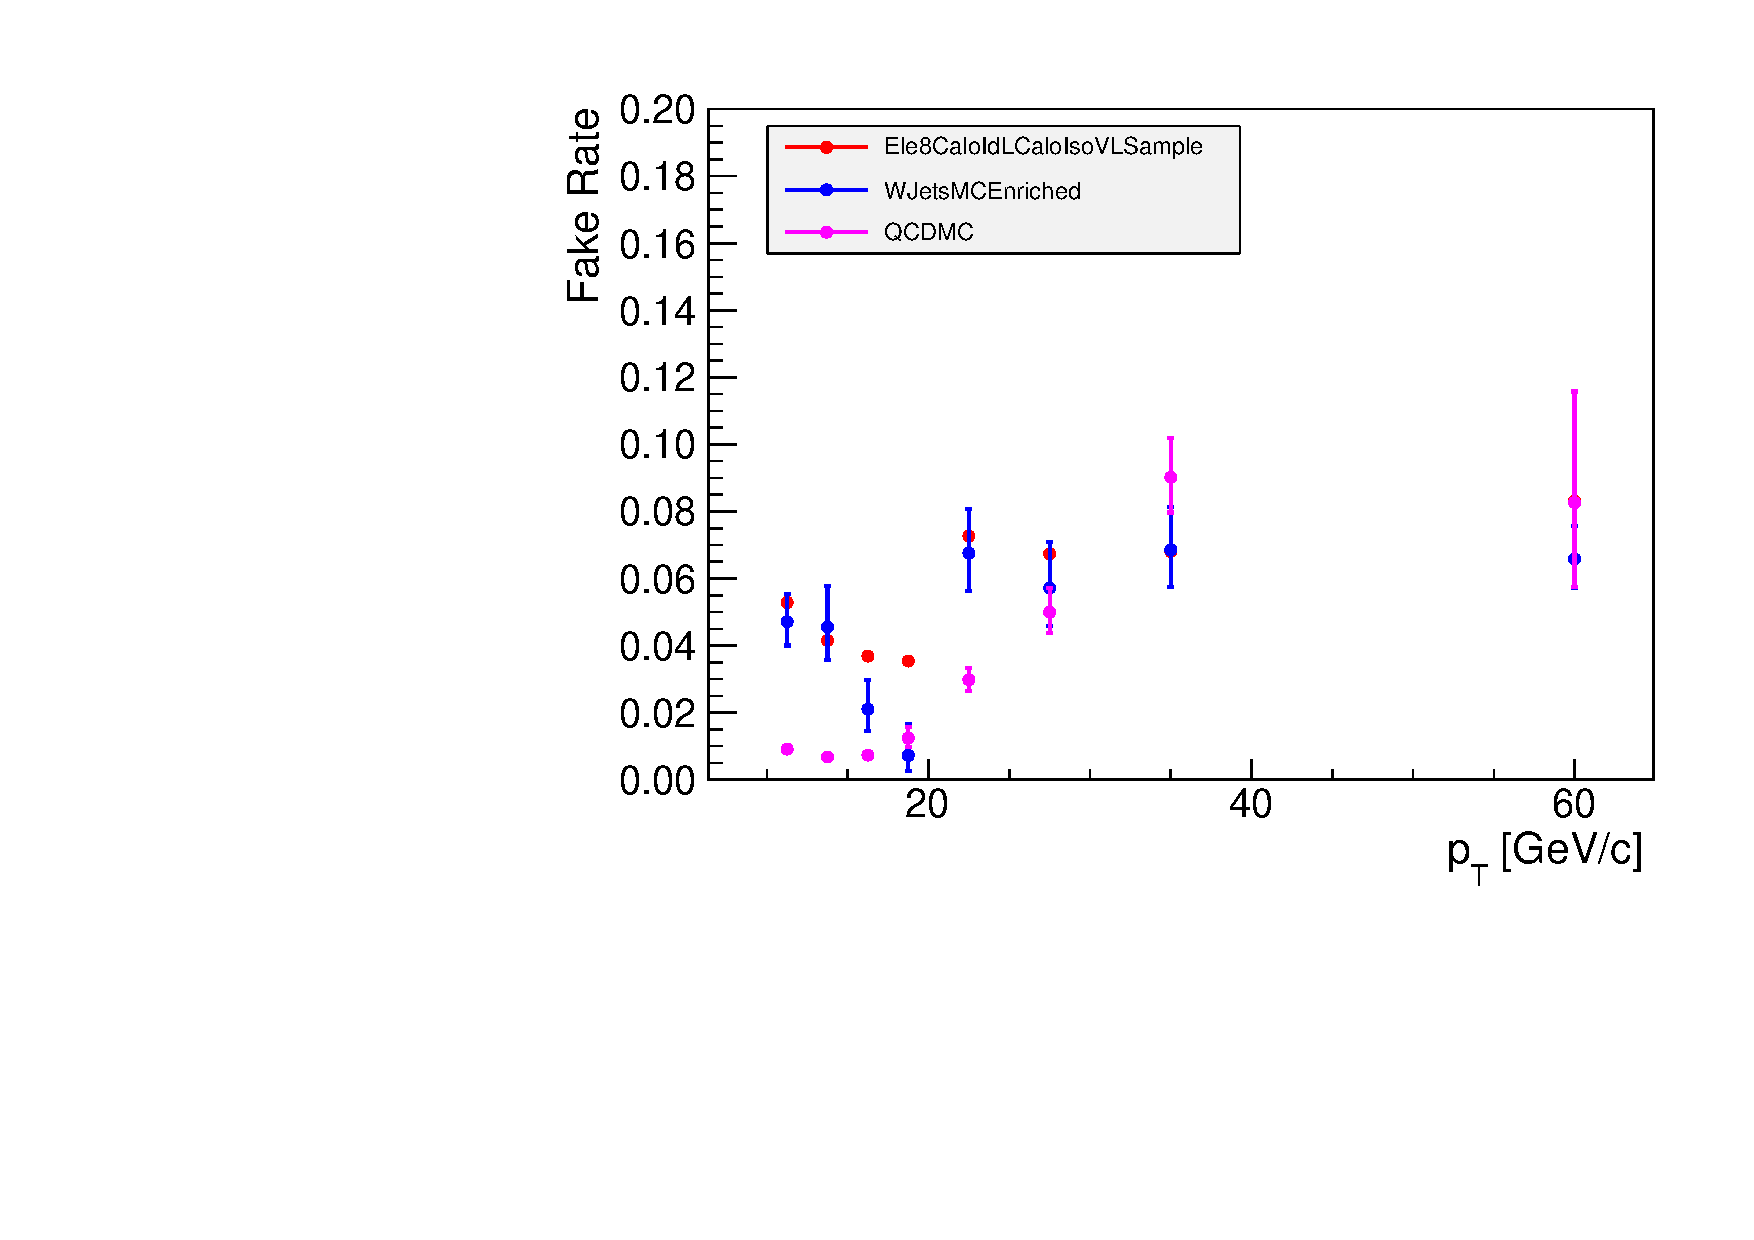
\includegraphics[width=0.45\textwidth]{figures/ElectronFakeRate_DenominatorV1_ptThreshold15_Pt.pdf}
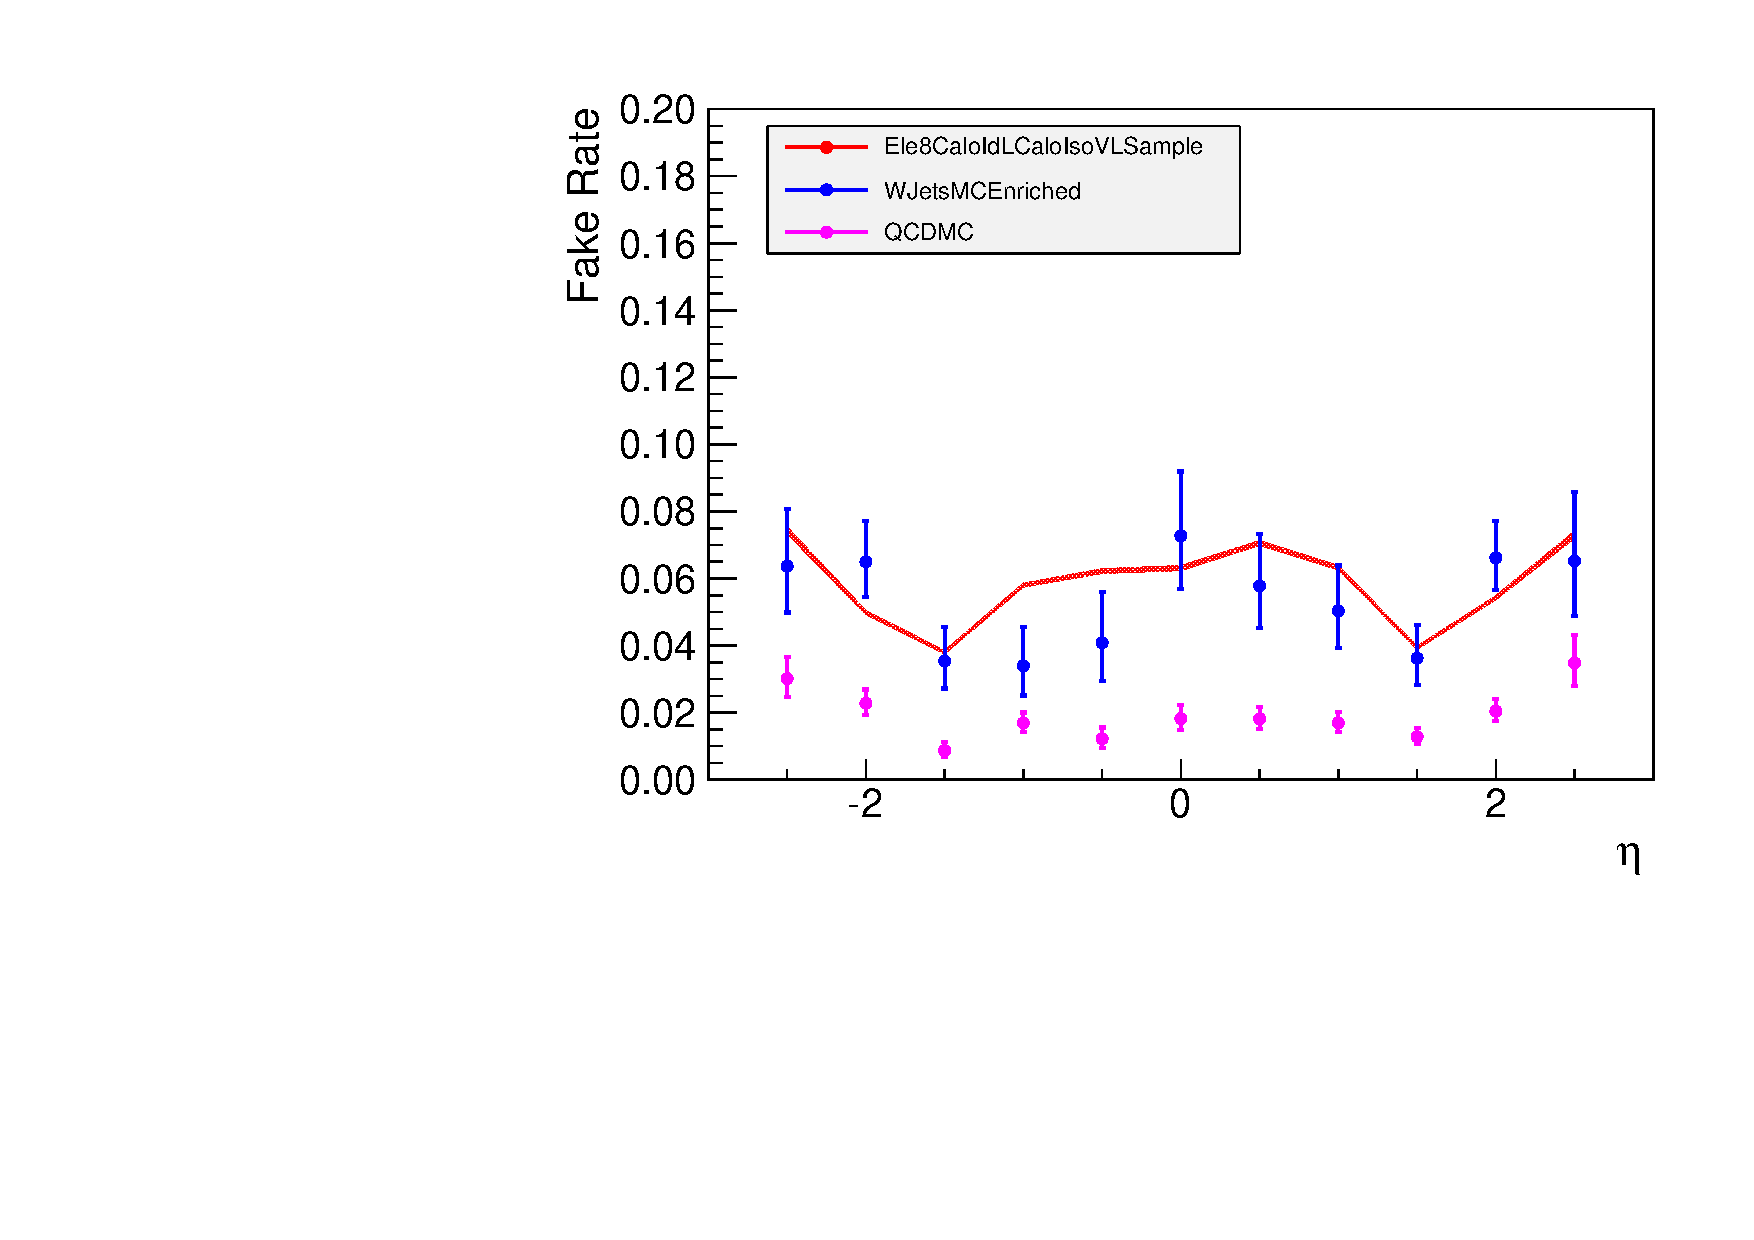
\includegraphics[width=0.45\textwidth]{figures/ElectronFakeRate_DenominatorV1_ptThreshold15_Eta.pdf}
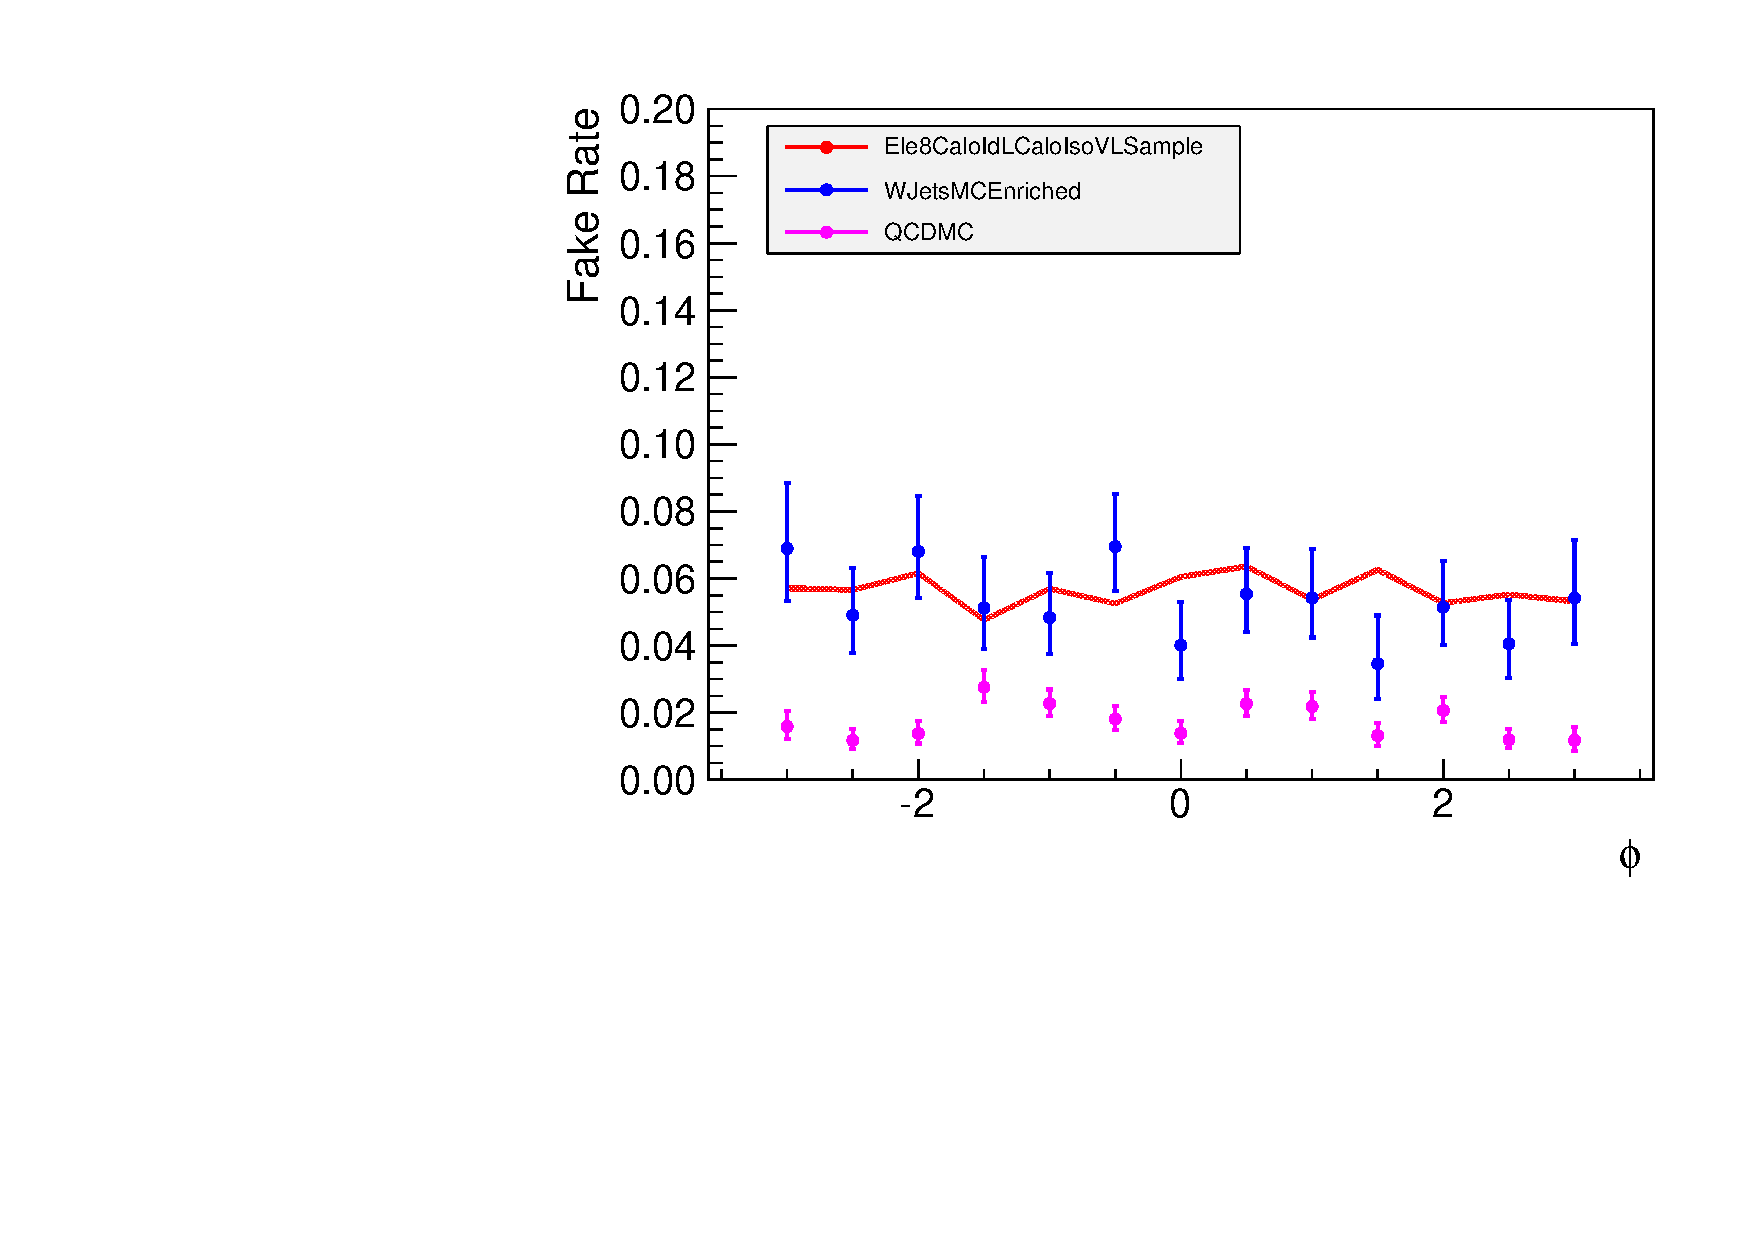
\includegraphics[width=0.45\textwidth]{figures/ElectronFakeRate_DenominatorV1_ptThreshold15_Phi.pdf}
\caption{Fake rates for V1 definition as a function of $p_T$,$\eta$, and $\phi$.}
\label{fig:ele_fr_V1_jet15}
\end{center}
\end{figure}

\begin{figure}[!htbp]
\begin{center}
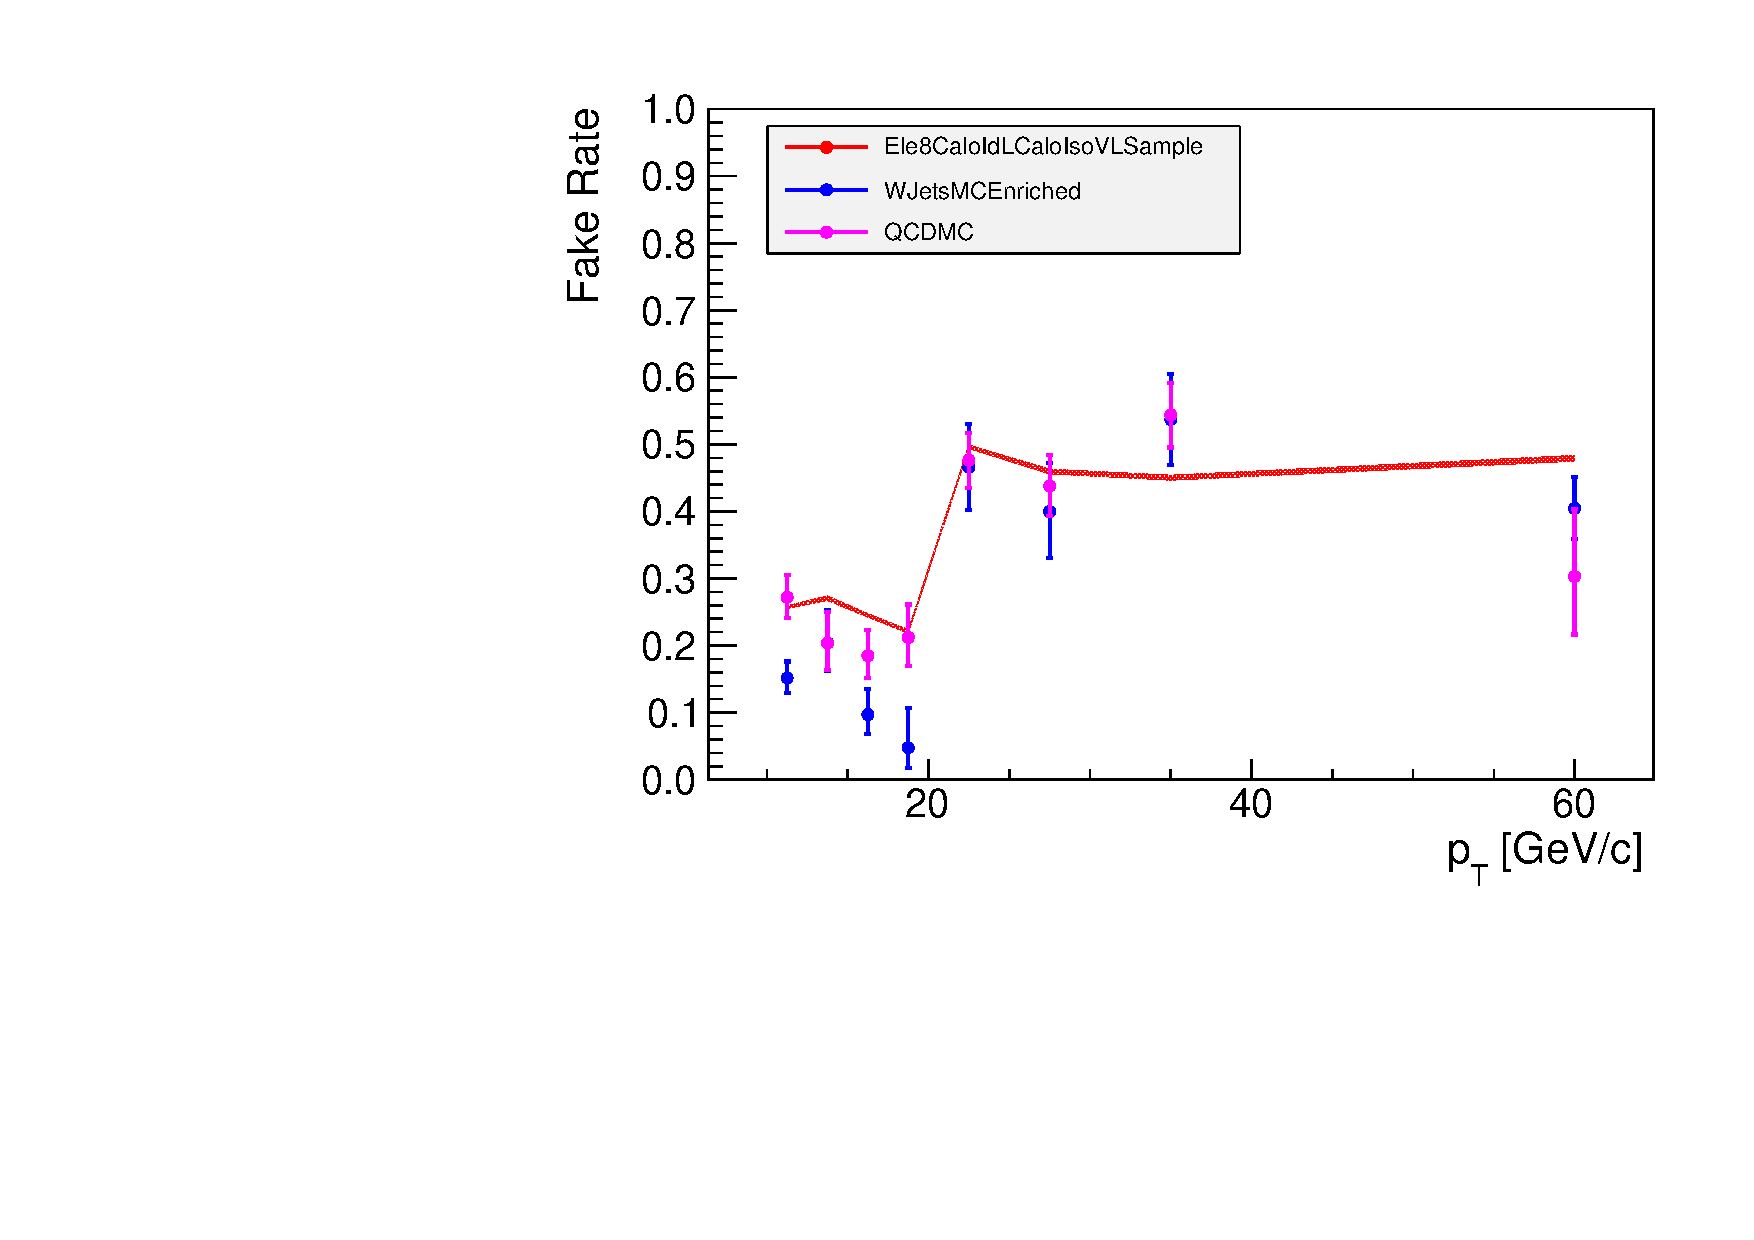
\includegraphics[width=0.45\textwidth]{figures/ElectronFakeRate_DenominatorV2_ptThreshold15_Pt.pdf}
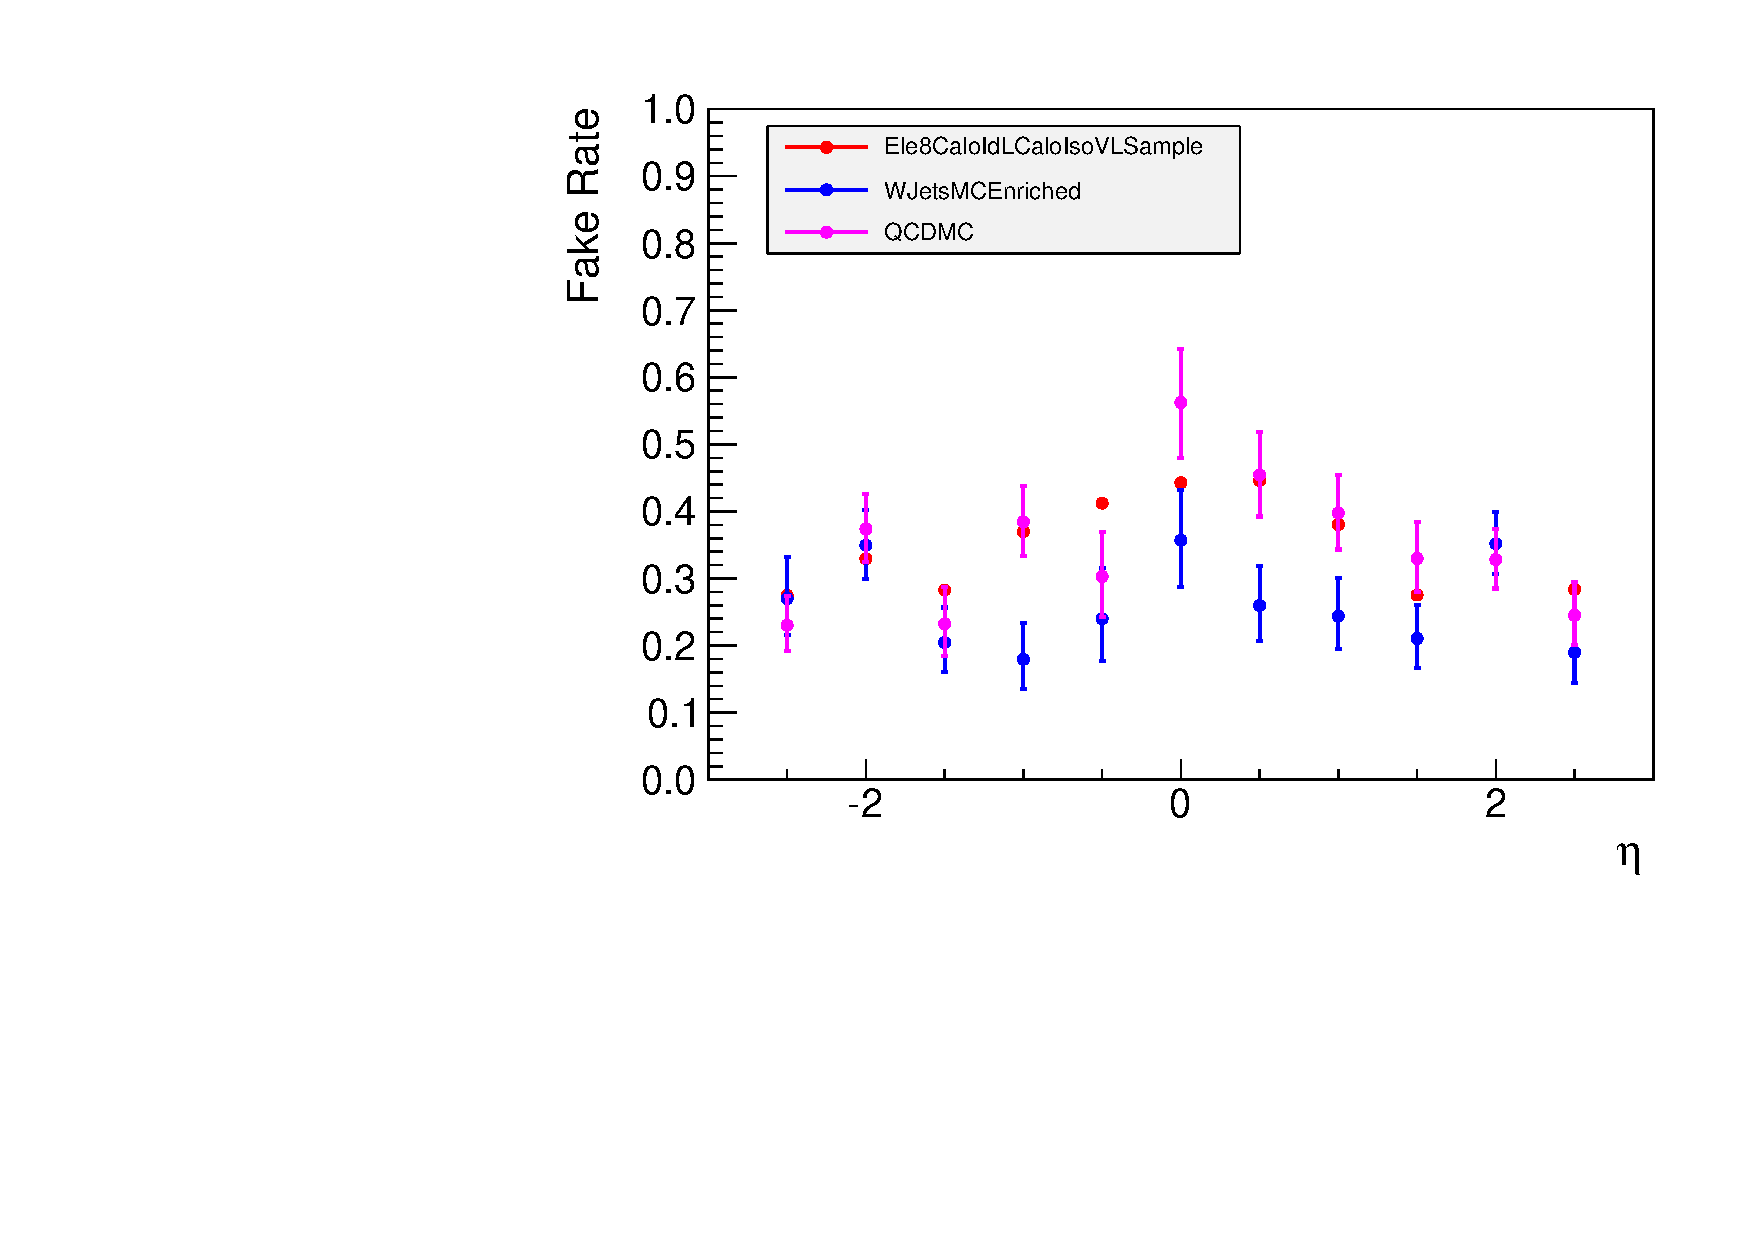
\includegraphics[width=0.45\textwidth]{figures/ElectronFakeRate_DenominatorV2_ptThreshold15_Eta.pdf}
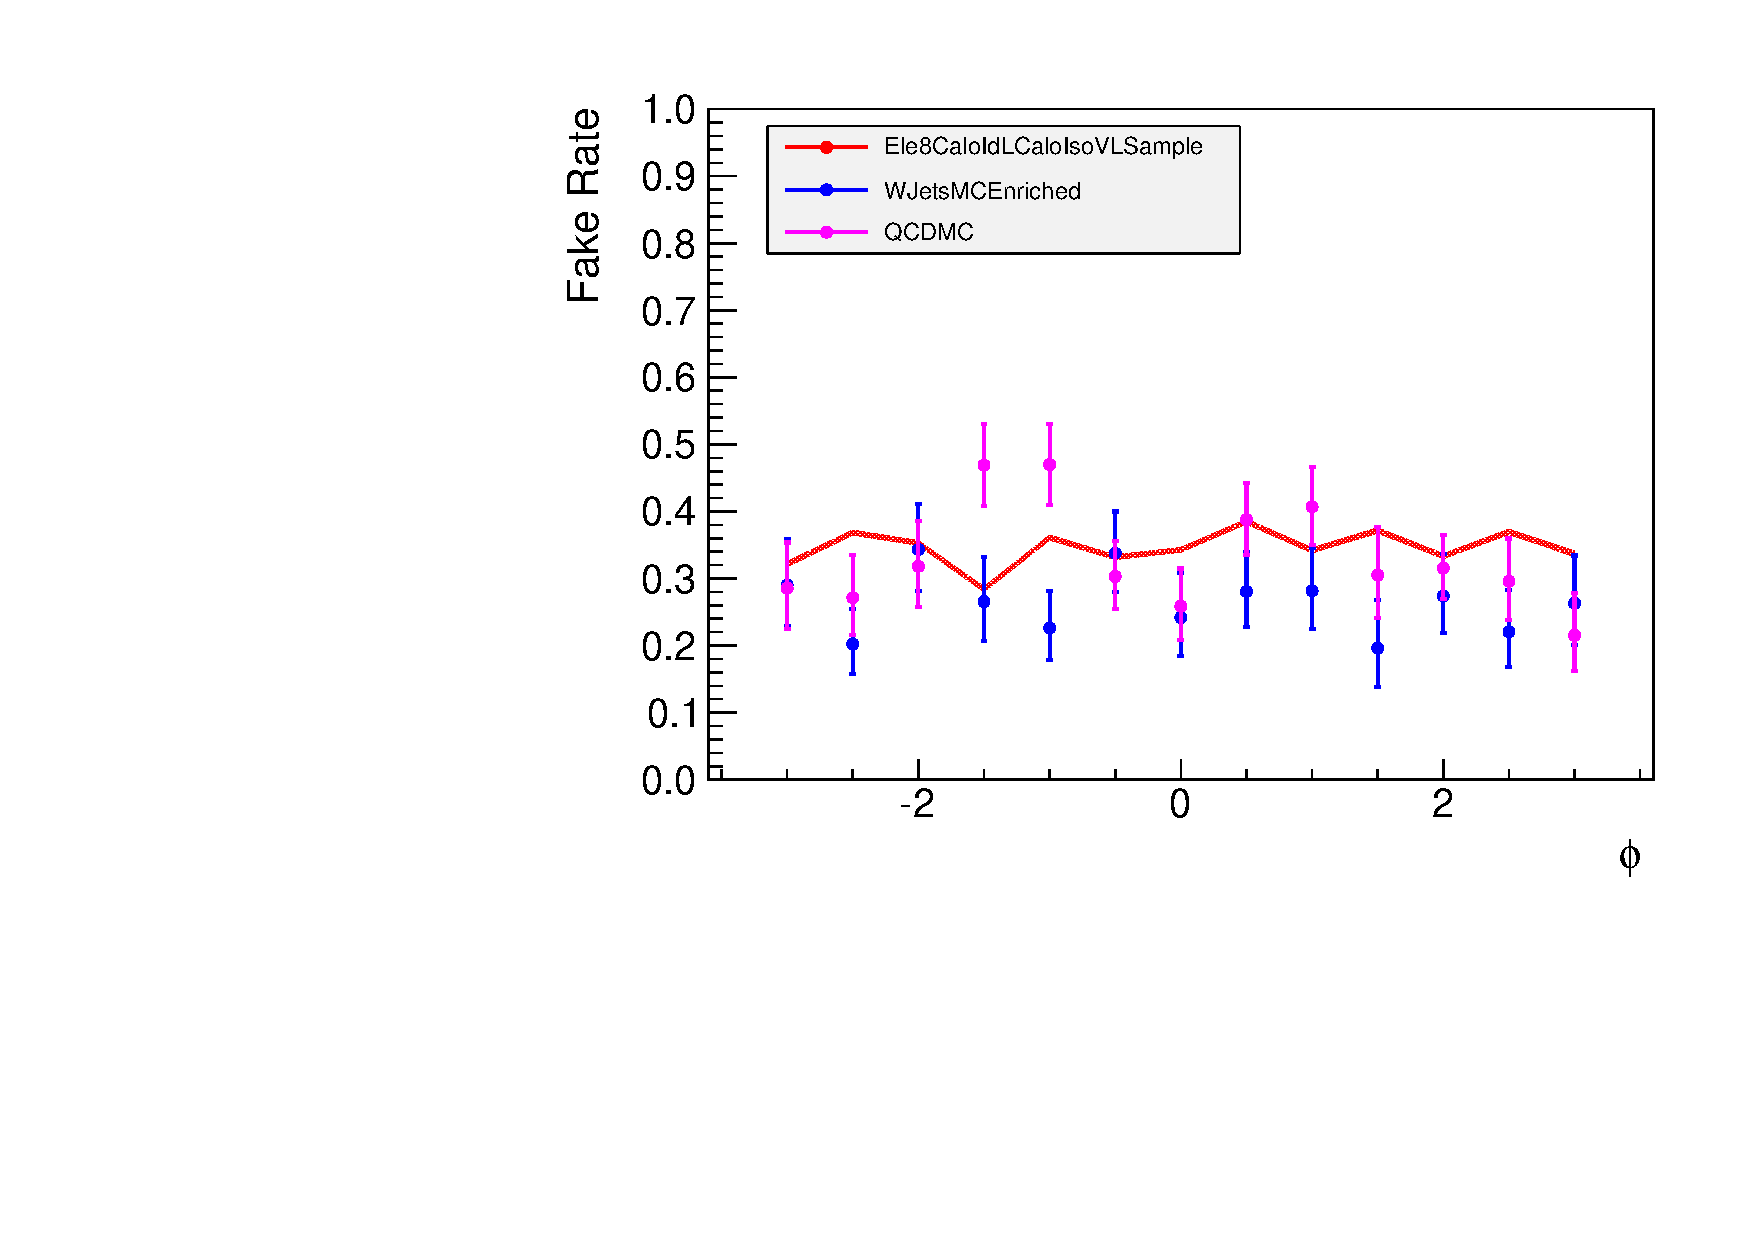
\includegraphics[width=0.45\textwidth]{figures/ElectronFakeRate_DenominatorV2_ptThreshold15_Phi.pdf}
\caption{Fake rates for V2 definition as a function of $p_T$,$\eta$, and $\phi$.}
\label{fig:ele_fr_V2_jet15}
\end{center}
\end{figure}

\begin{figure}[!htbp]
\begin{center}
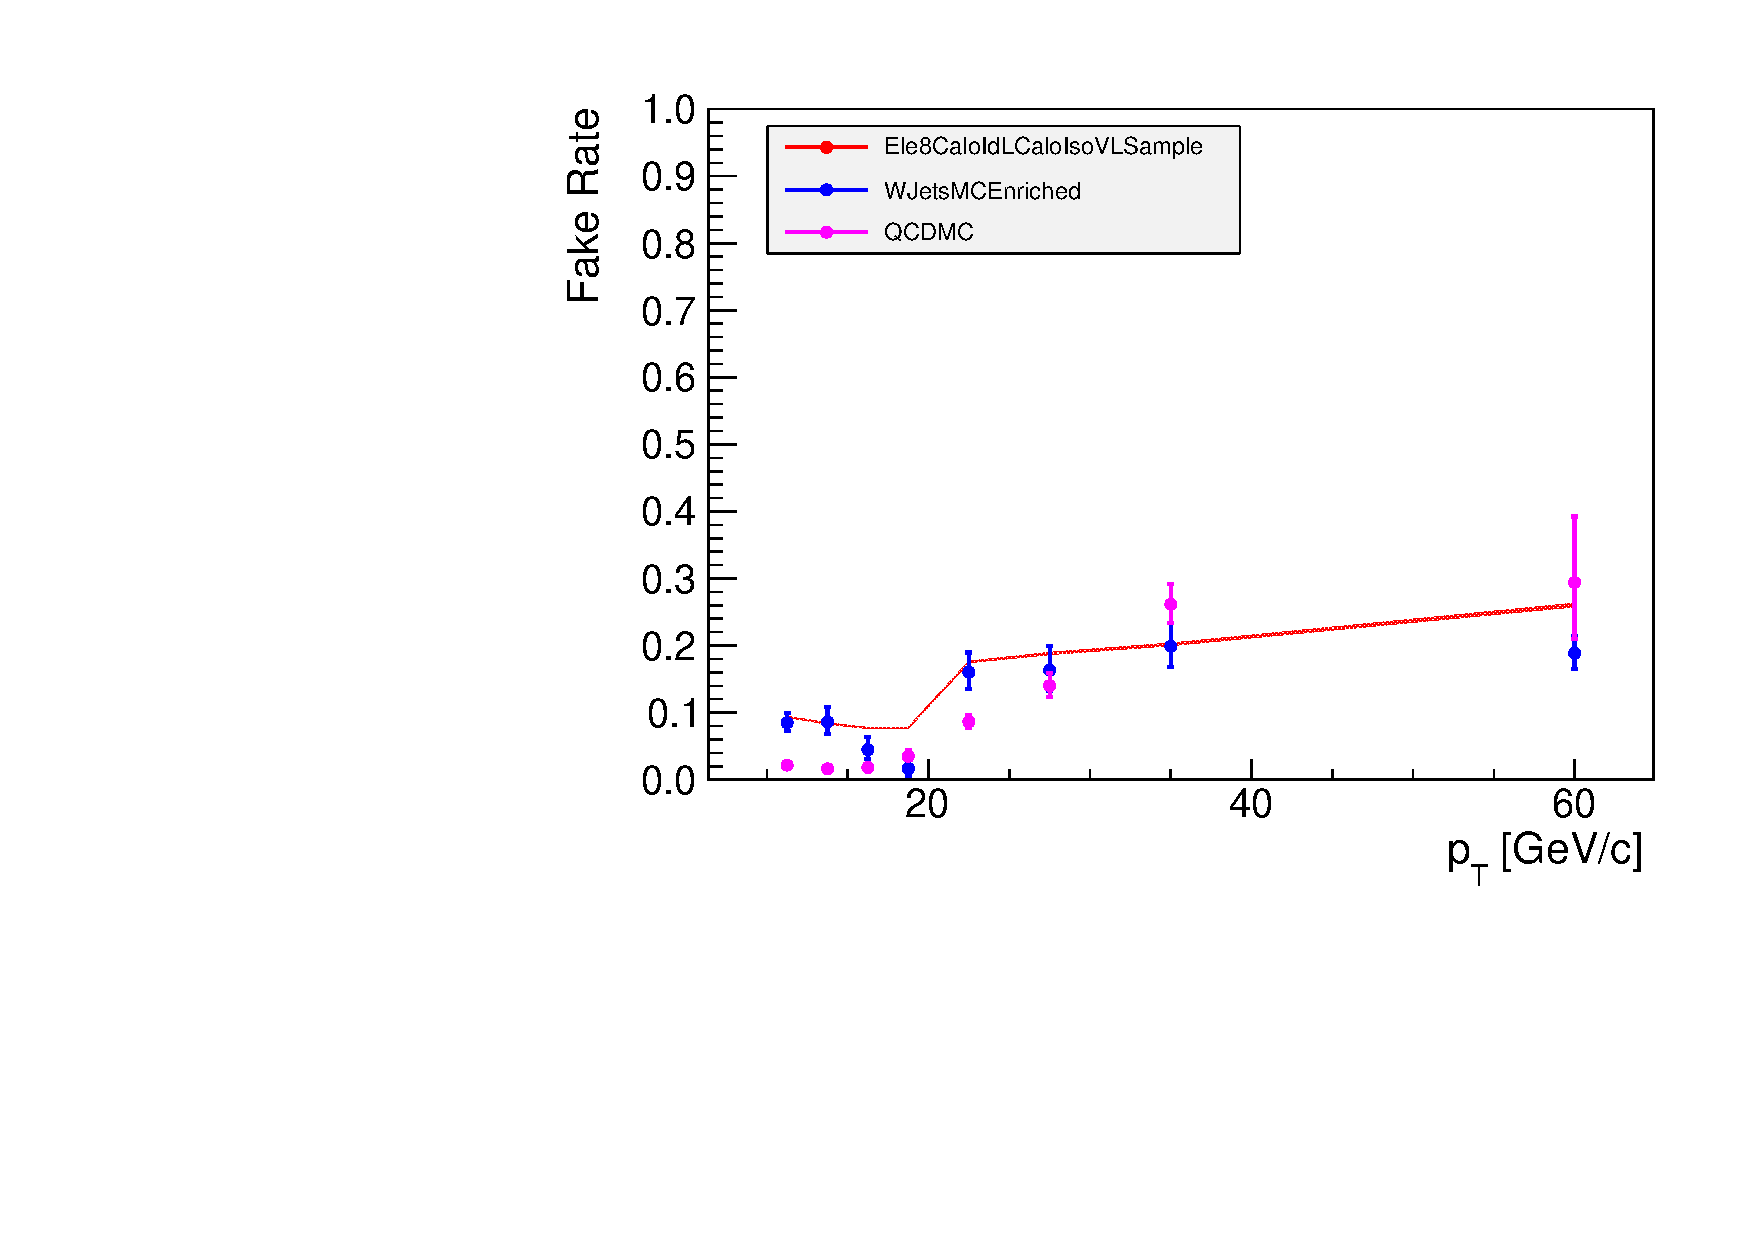
\includegraphics[width=0.45\textwidth]{figures/ElectronFakeRate_DenominatorV3_ptThreshold15_Pt.pdf}
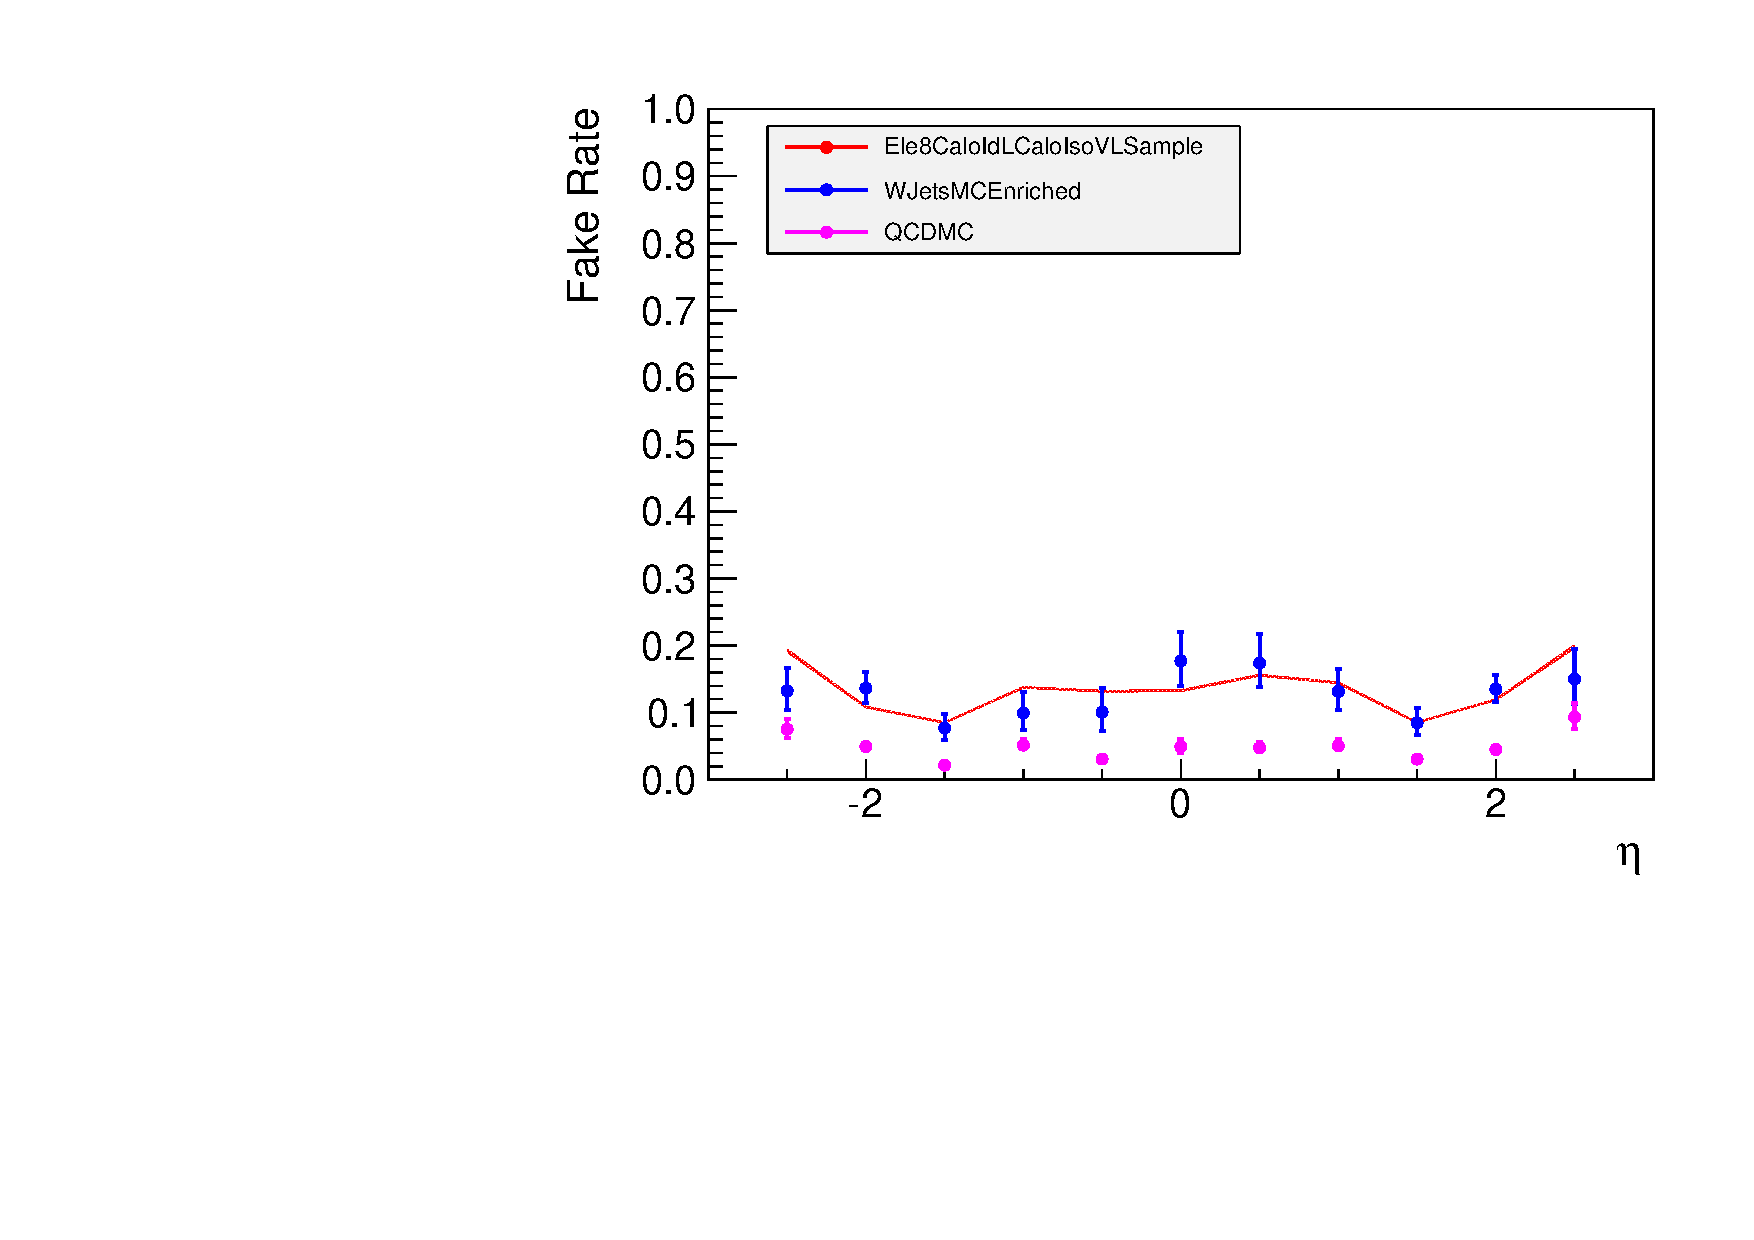
\includegraphics[width=0.45\textwidth]{figures/ElectronFakeRate_DenominatorV3_ptThreshold15_Eta.pdf}
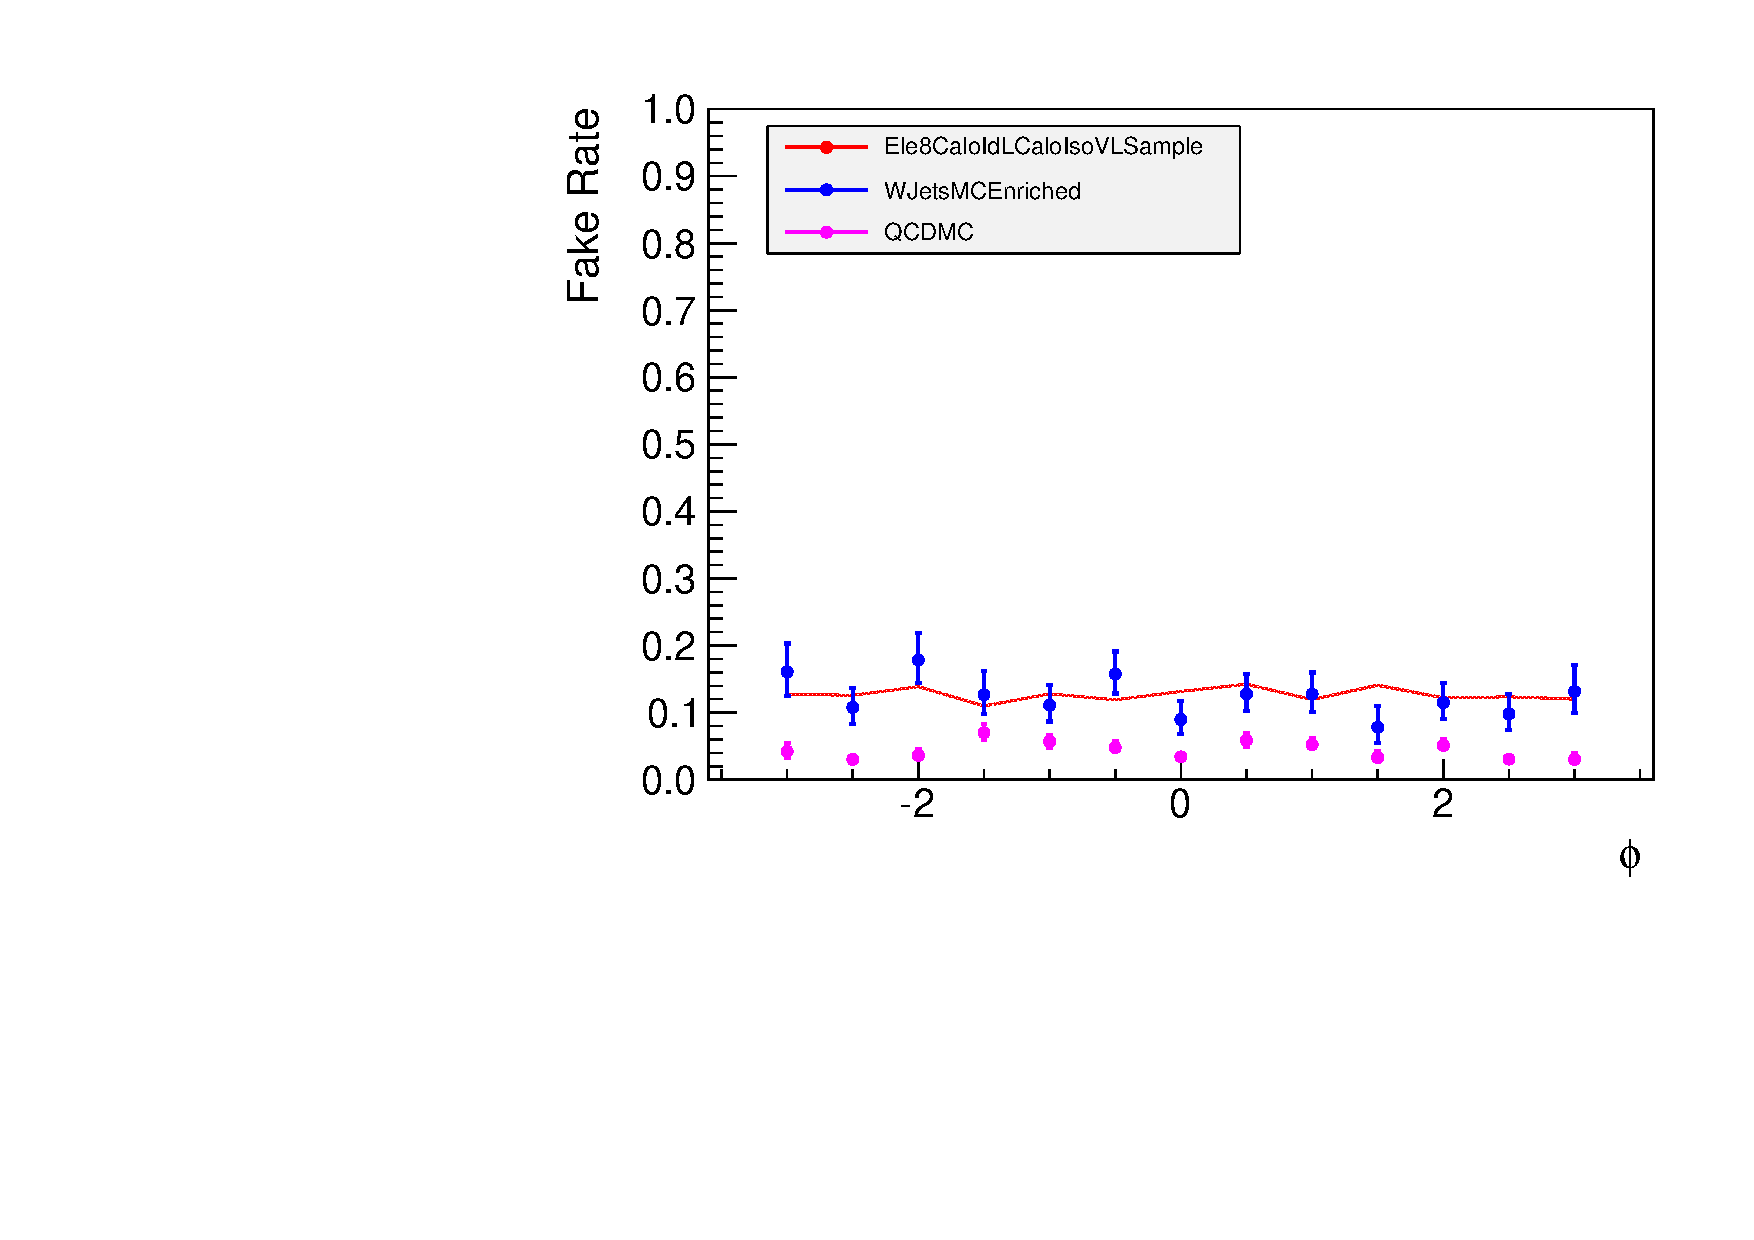
\includegraphics[width=0.45\textwidth]{figures/ElectronFakeRate_DenominatorV3_ptThreshold15_Phi.pdf}
\caption{Fake rates for V3 definition as a function of $p_T$,$\eta$, and $\phi$.}
\label{fig:ele_fr_V3_jet15}
\end{center}
\end{figure}

\begin{figure}[!htbp]
\begin{center}
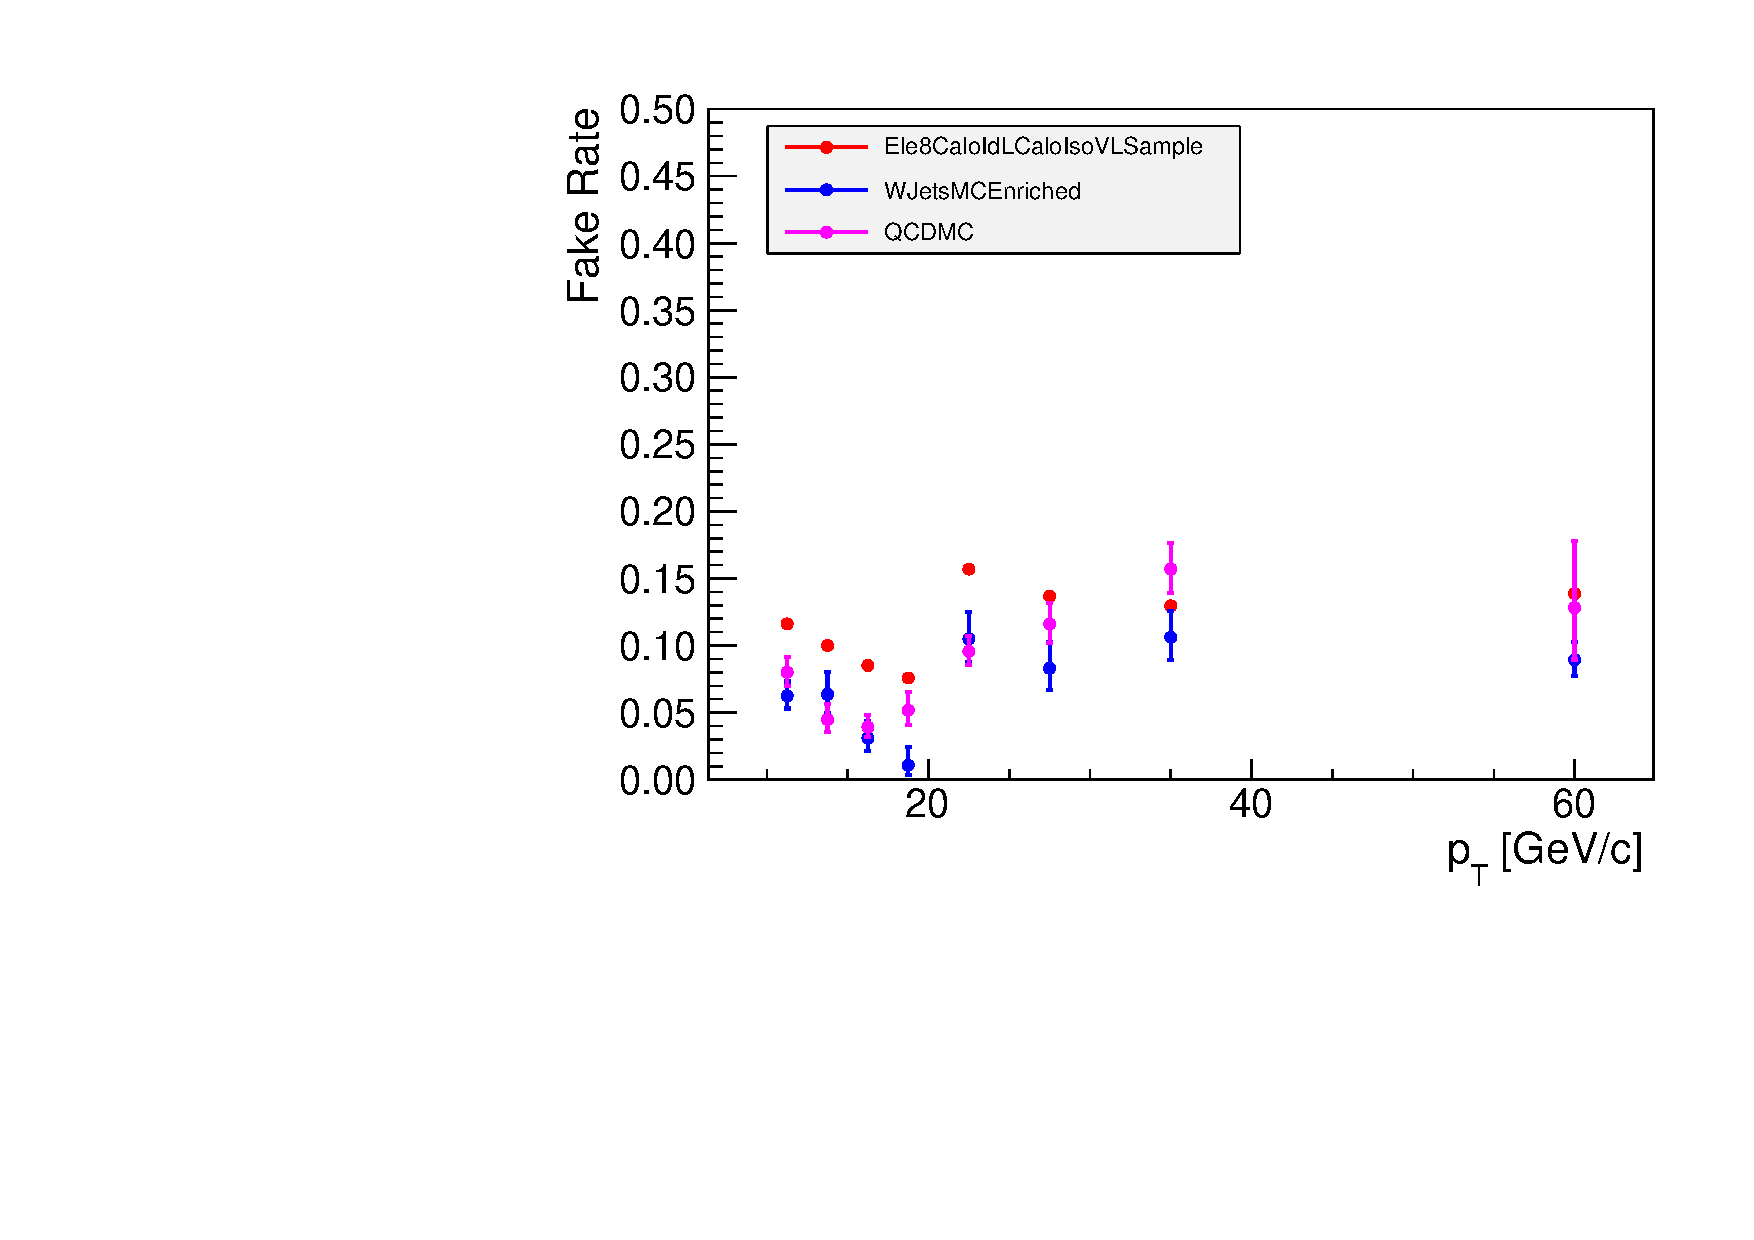
\includegraphics[width=0.45\textwidth]{figures/ElectronFakeRate_DenominatorV4_ptThreshold15_Pt.pdf}
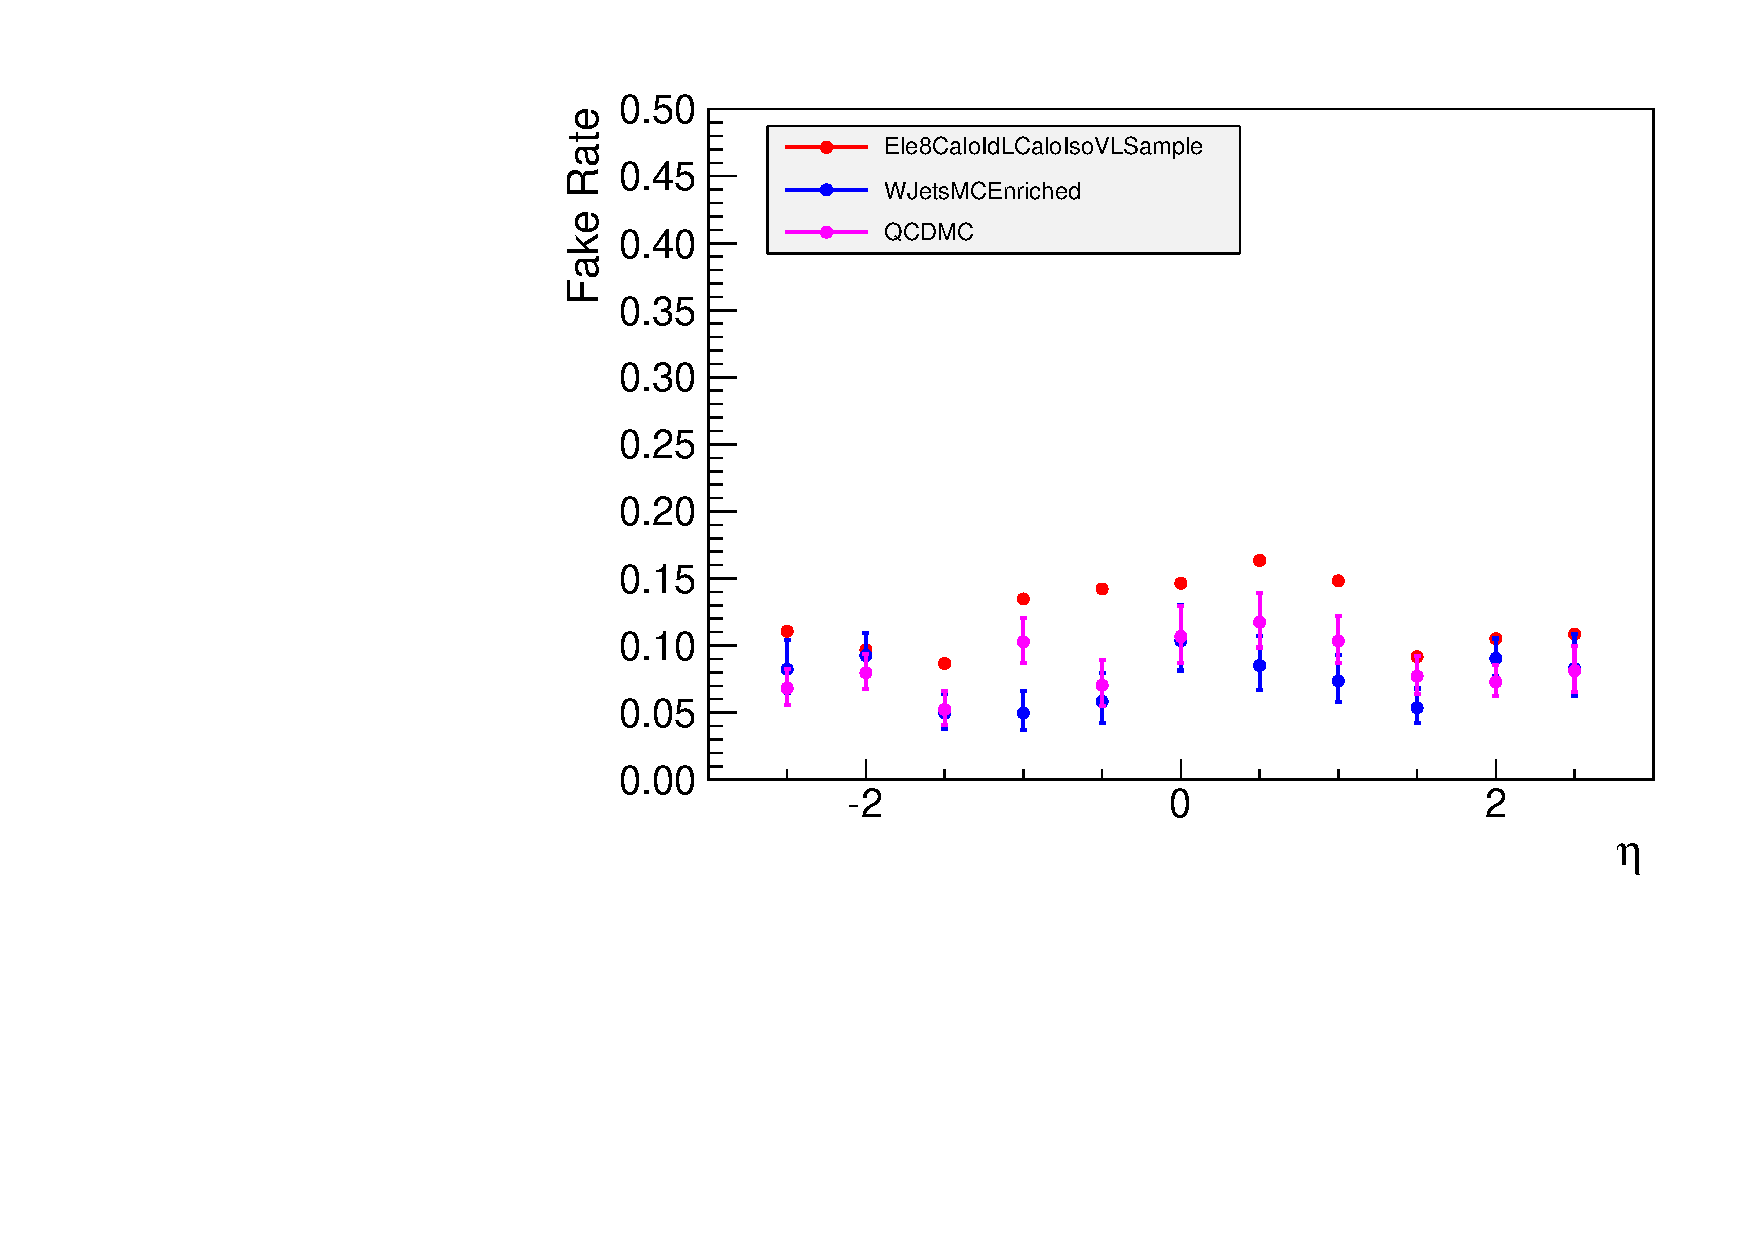
\includegraphics[width=0.45\textwidth]{figures/ElectronFakeRate_DenominatorV4_ptThreshold15_Eta.pdf}
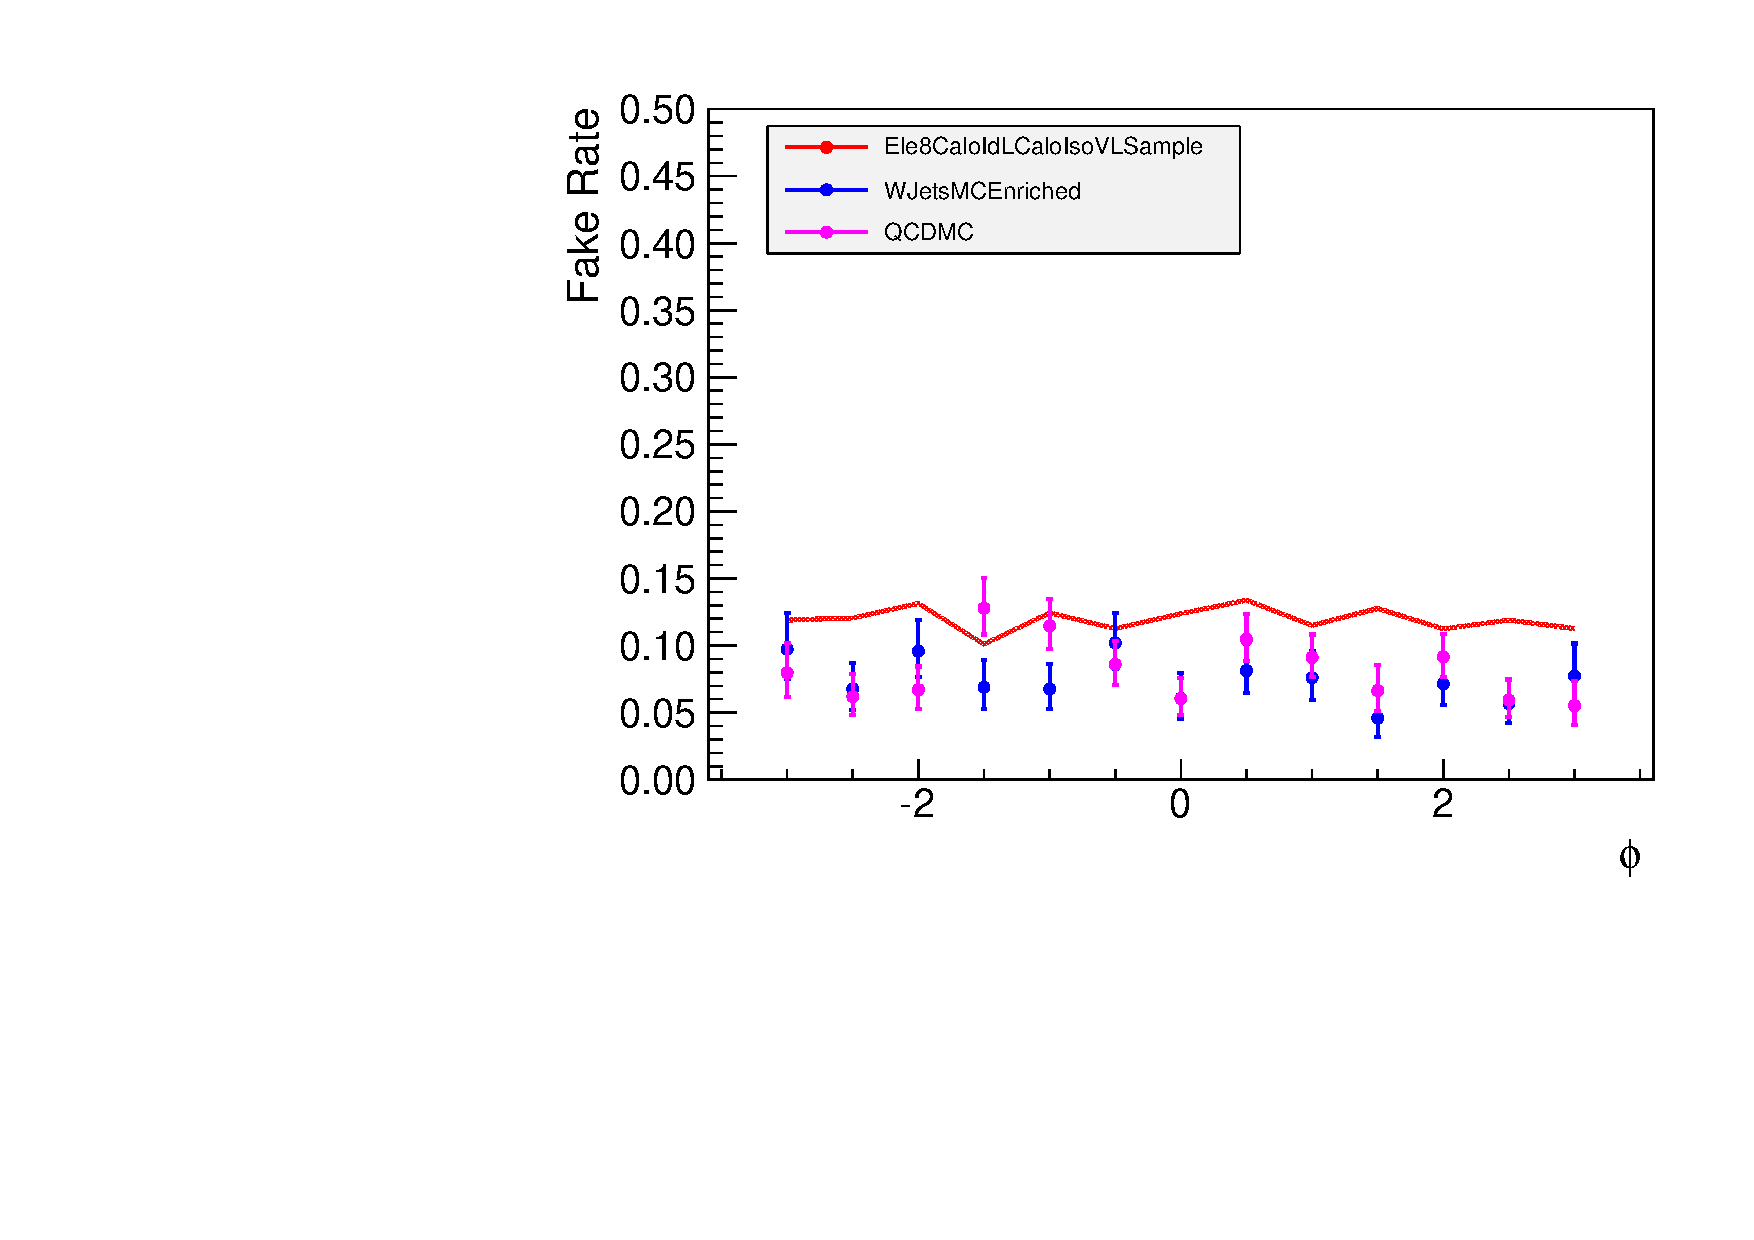
\includegraphics[width=0.45\textwidth]{figures/ElectronFakeRate_DenominatorV4_ptThreshold15_Phi.pdf}
\caption{Fake rates for V4 definition as a function of $p_T$,$\eta$, and $\phi$.}
\label{fig:ele_fr_V4_jet15}
\end{center}
\end{figure}

Due to the fact that the Monte Carlo simulation does not have an implementation of the trigger used
to collect the fake electron candidates, it is expected that the Monte Carlo fake rate will differ
from the data fake rates. The V2 fake rate is expected to give better agreement between data and 
Monte Carlo simulation, since the denominator is already fully isolated. For $p_{T} > 20$ GeV, 
the fake rate from QCD Monte Carlo actually gives a reasonable description of the data. The difference
between the QCD Monte Carlo and the W+Jet Monte Carlo fake rate reflects the systematic uncertainties
due to different fake composition.


\subsubsection{Systematics}
To study the systematic uncertainty due to the jet $p_{T}$ spectrum, we compare the fake rates
measured requiring different thresholds on the $p_{T}$ of the leading jet. The comparisons
are shown in Fig \ref{fig:ele_fr_jetPtThresholdDependence} for the different denominator definitions. 
In Table~\ref{tab:ele_fr_ptThreshold_dep} we summarize the systematic uncertainty due to 
the jet $p_{T}$ uncertainty, obtained by taking the largest relative difference between 
the fake rates measured in the jet0, jet15, and jet30 samples.

\begin{table}[!htbp]
\begin{center}
\begin{tabular}{|c|cc|c|}
\hline
FO & $p_T<20$ & $p_T>20$ & Overall \\
\hline 
V1 & $47\%$ & $39\%$ & $36\%$ \\
V2 & $12\%$ & $9\%$ & $12\%$ \\
V3 & $38\%$ & $32\%$ & $24\%$ \\
V4 & $16\%$ & $29\%$ & $17\%$ \\
\hline
\end{tabular}
\caption{Systematic uncertainties due to jet $p_{T}$ spectrum uncertainty.}
\label{tab:ele_fr_ptThreshold_dep}
\end{center}
\end{table}


\begin{figure}[!htbp]
\begin{center}
\subfigure[V1 Denominator]{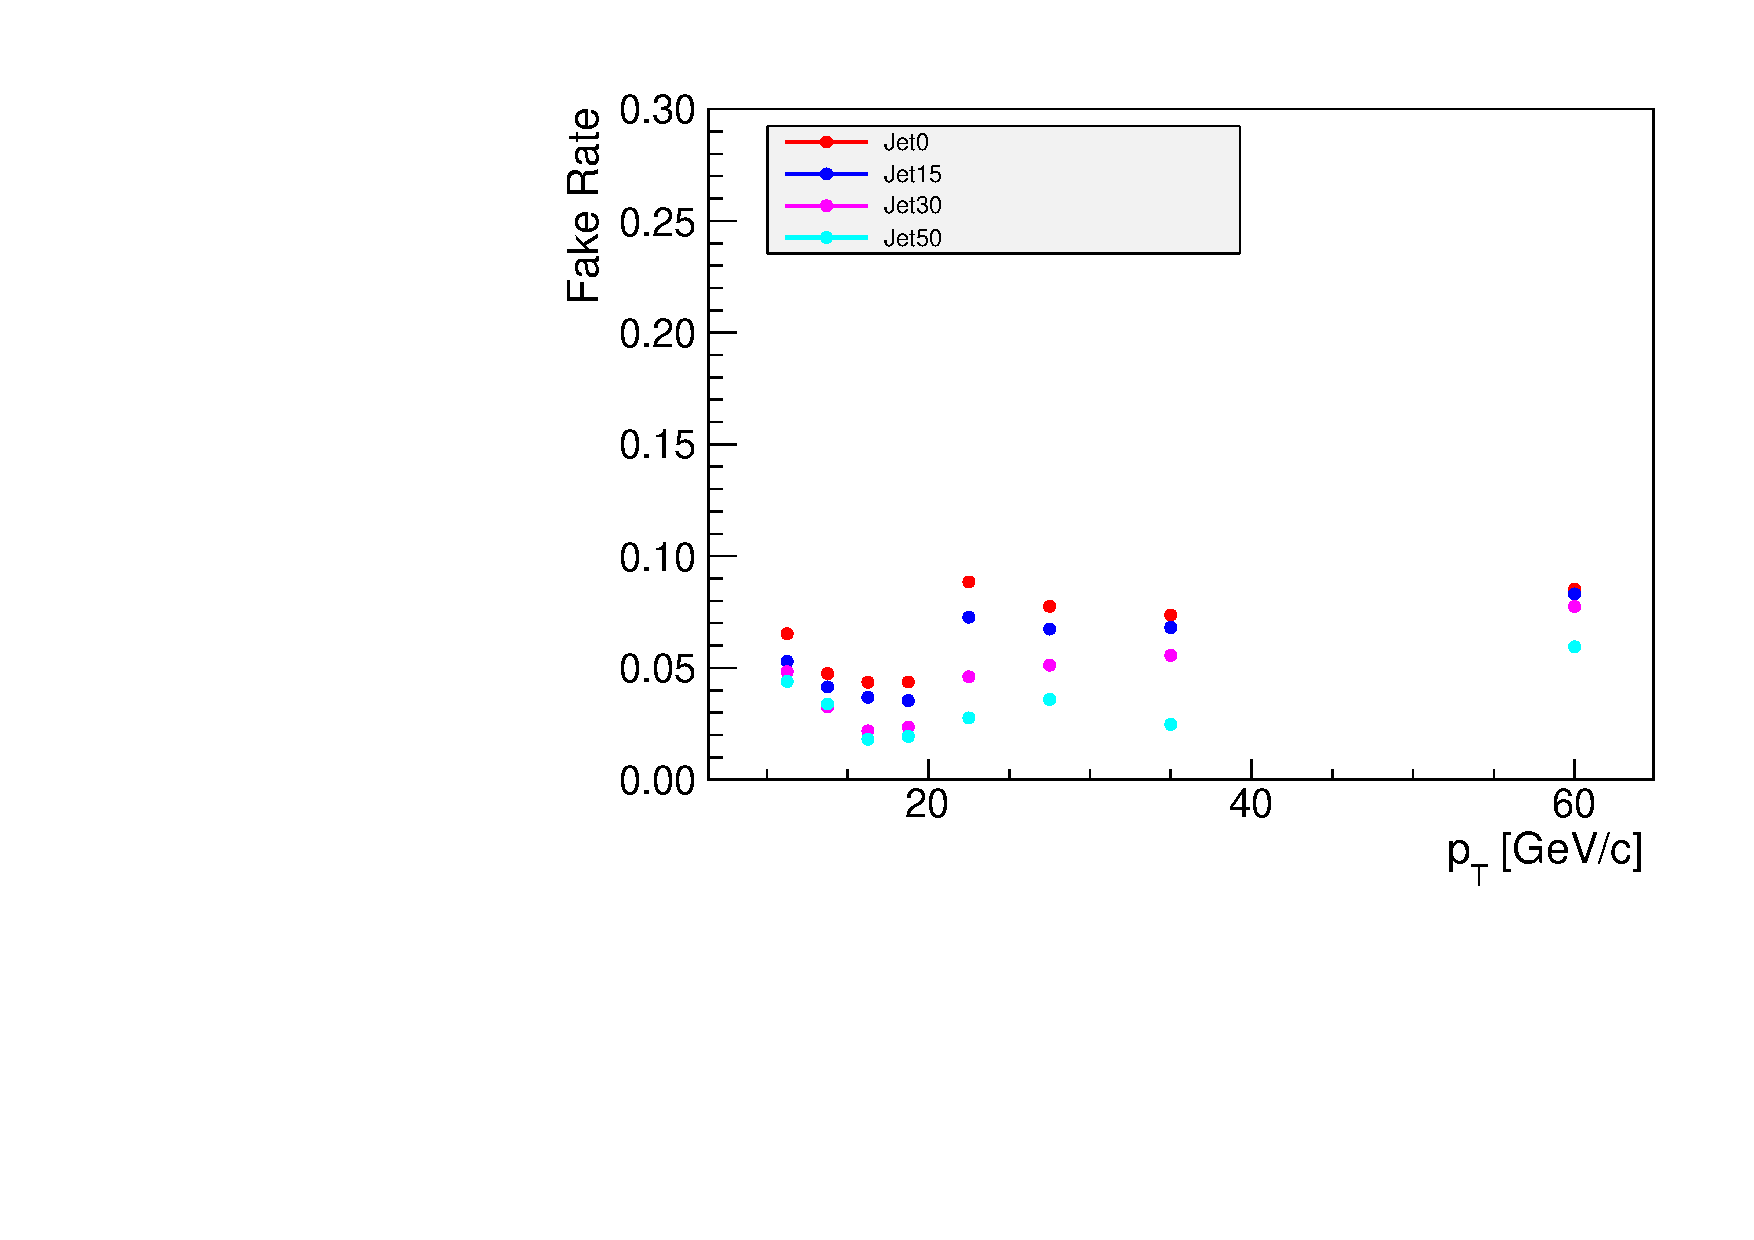
\includegraphics[width=0.45\textwidth]{figures/ElectronFakeRate_DenominatorV1_Ele8CaloIdLCaloIsoVLSample_Pt.pdf}}
\subfigure[V2 Denominator]{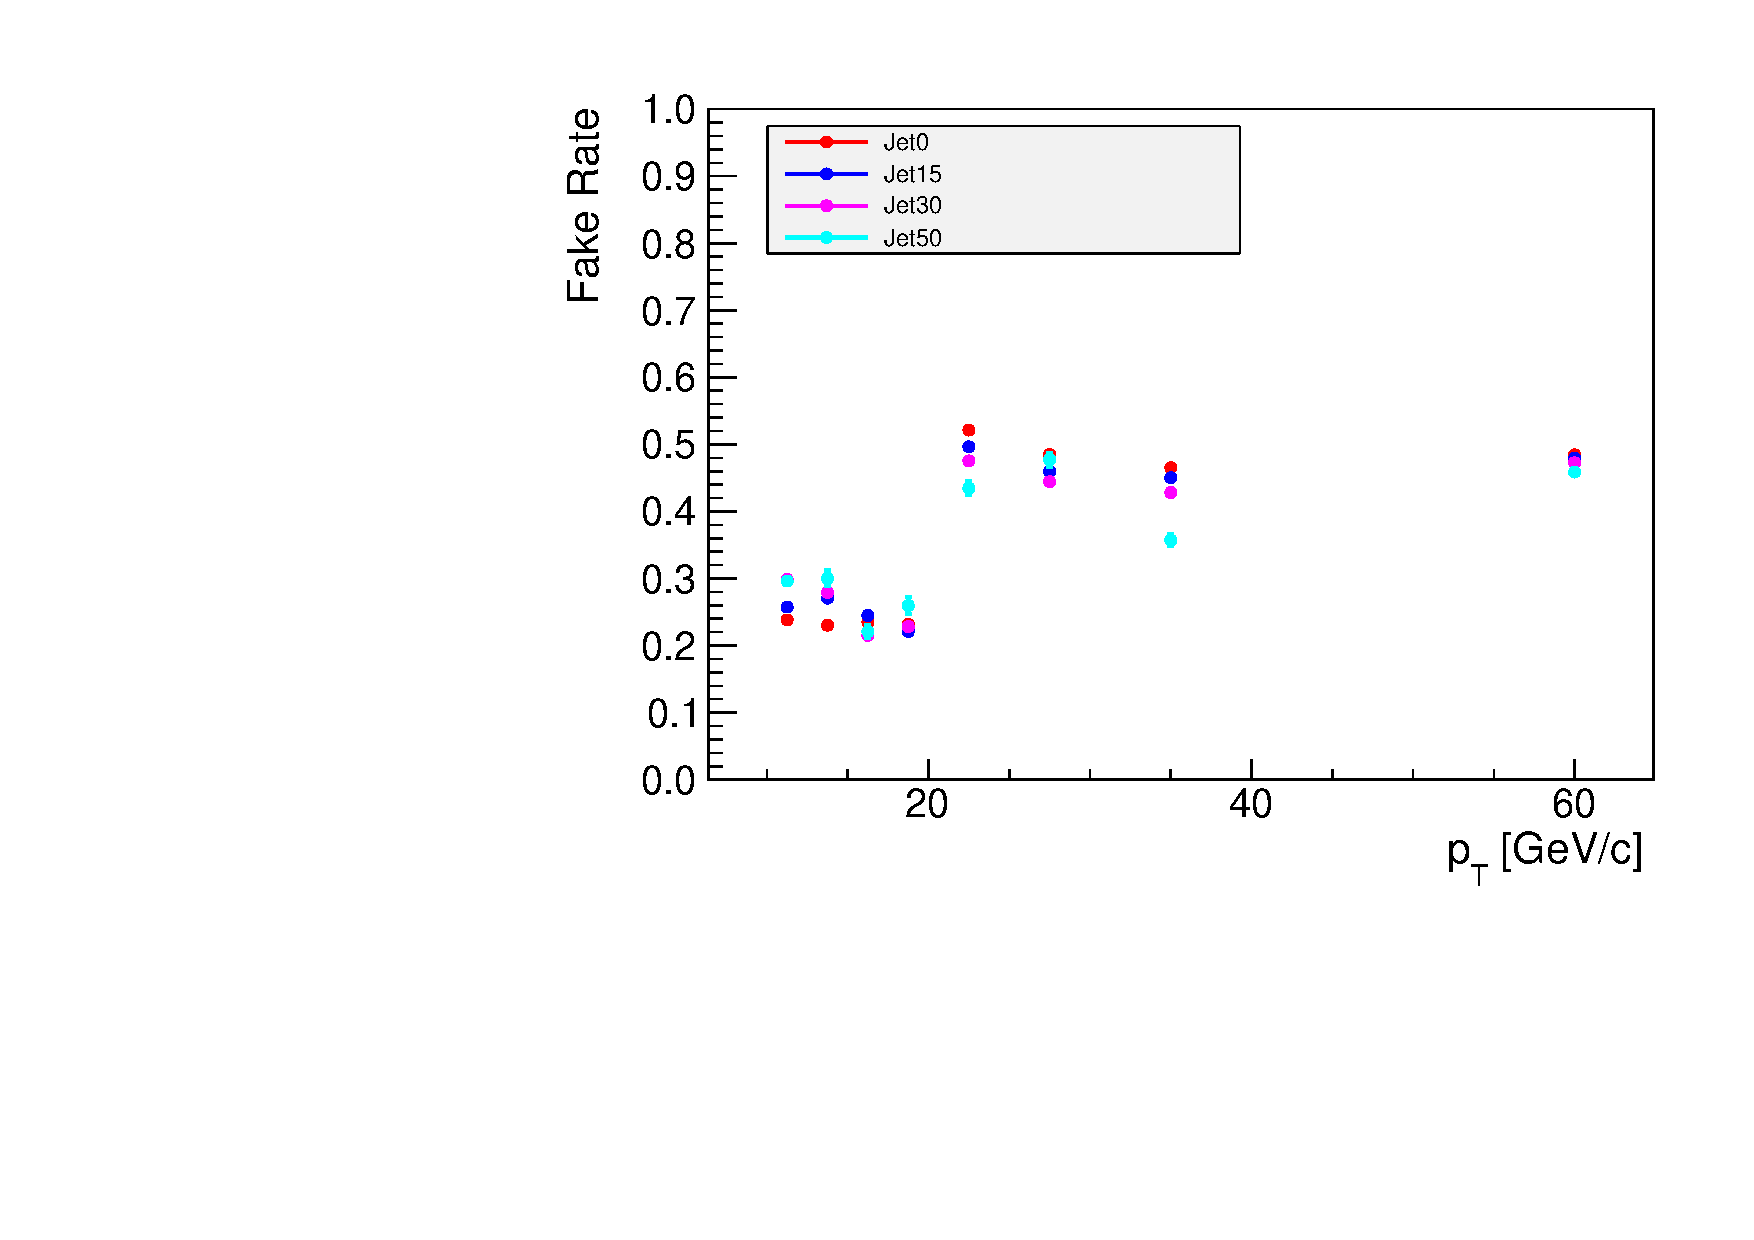
\includegraphics[width=0.45\textwidth]{figures/ElectronFakeRate_DenominatorV2_Ele8CaloIdLCaloIsoVLSample_Pt.pdf}}
\subfigure[V3 Denominator]{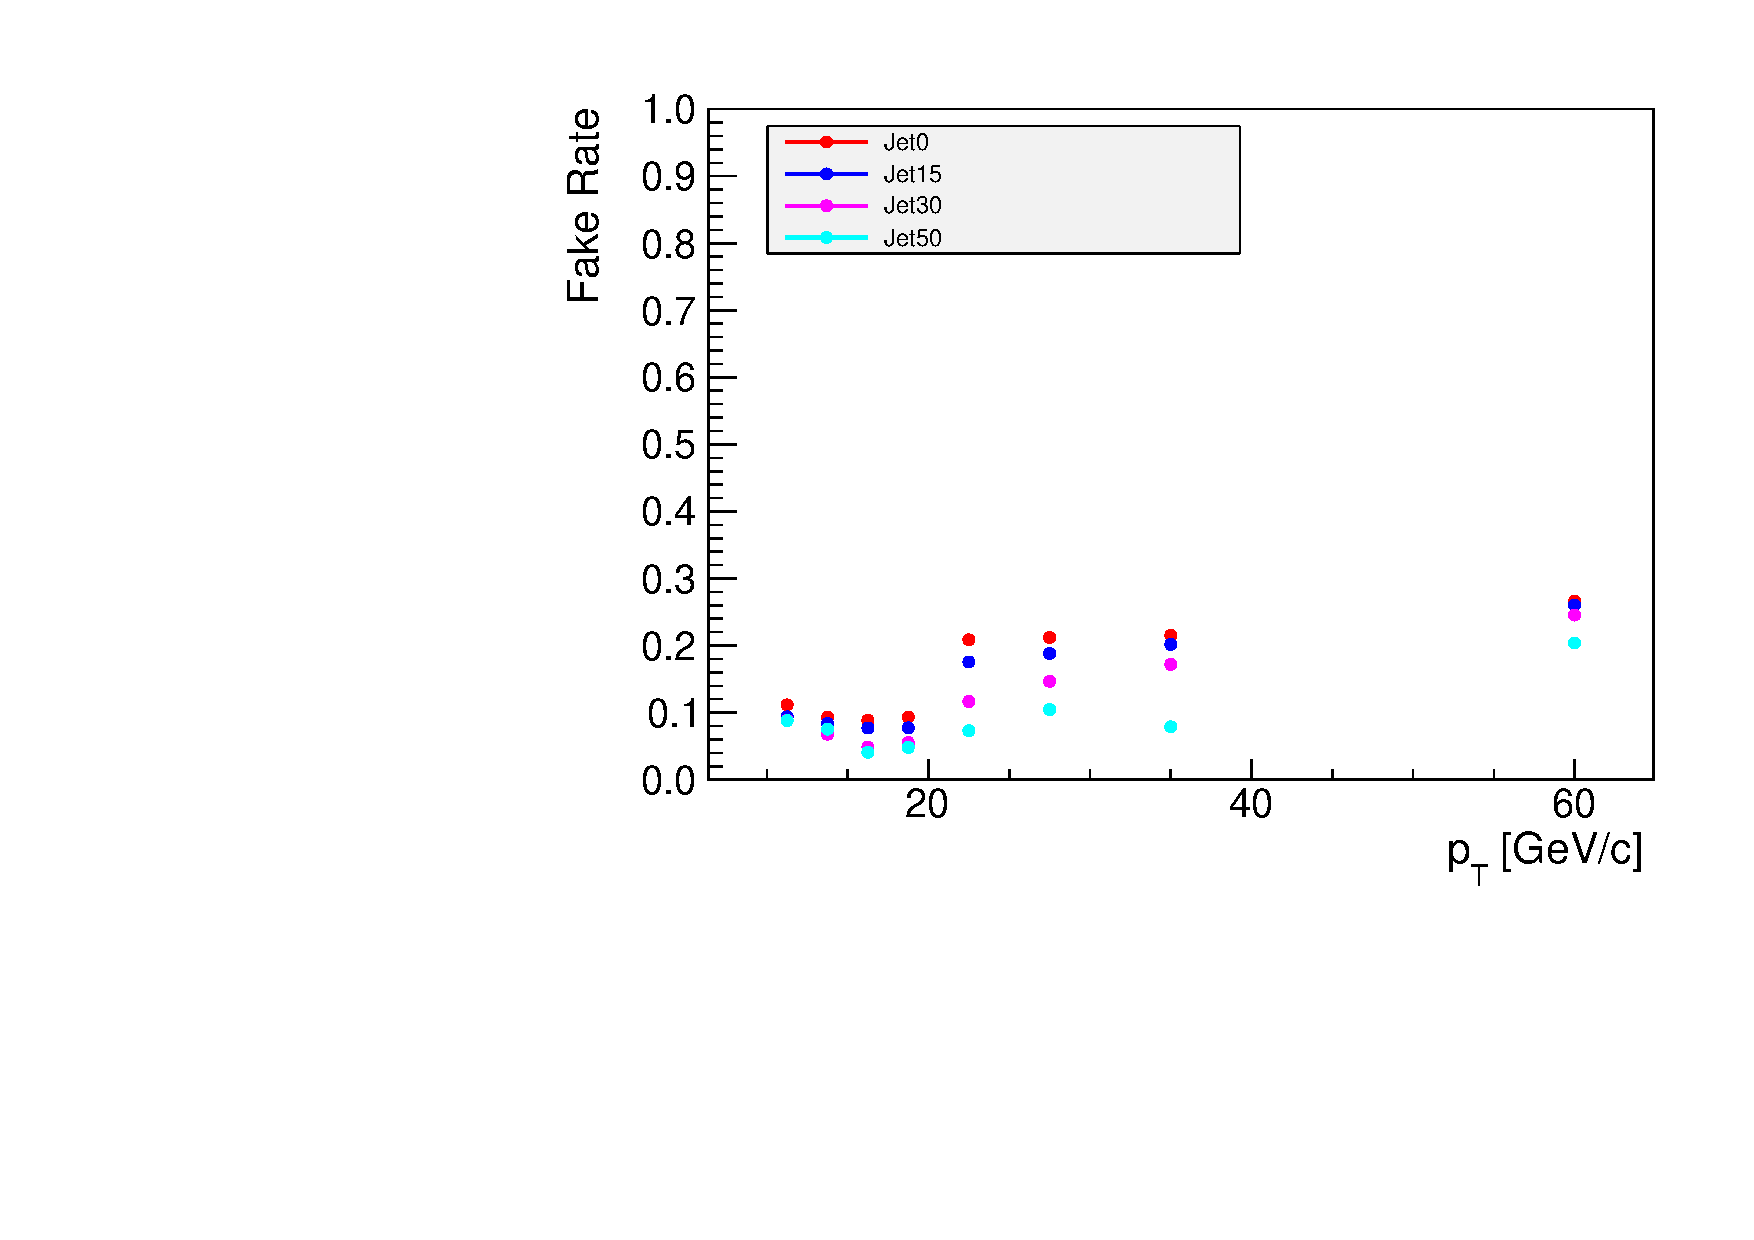
\includegraphics[width=0.45\textwidth]{figures/ElectronFakeRate_DenominatorV3_Ele8CaloIdLCaloIsoVLSample_Pt.pdf}}
\subfigure[V4 Denominator]{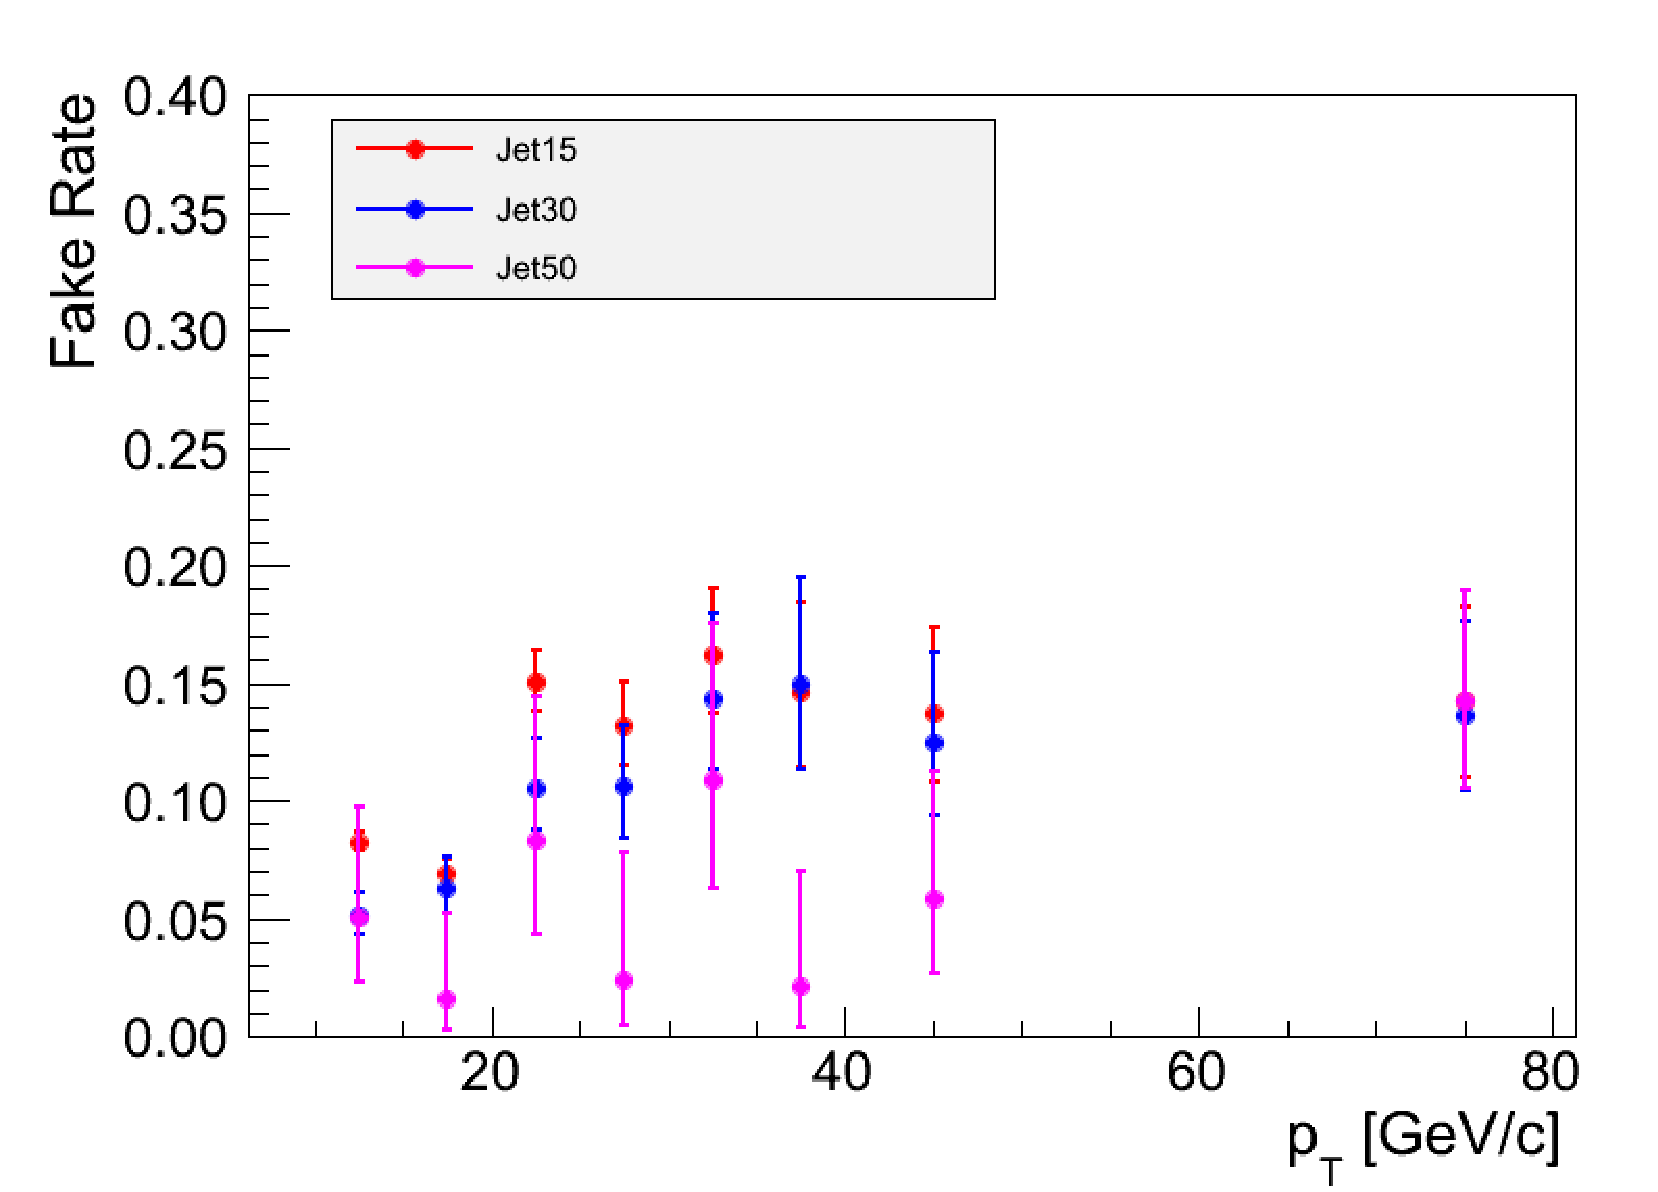
\includegraphics[width=0.45\textwidth]{figures/ElectronFakeRate_DenominatorV4_Ele8CaloIdLCaloIsoVLSample_Pt.pdf}}
\caption{Fake rates for the different fakeable object definitions, as a function of $p_T$, showing
the dependence on the $p_{T}$ threshold of the leading jet in the event.}
\label{fig:ele_fr_jetPtThresholdDependence}
\end{center}
\end{figure}

Due to the fact that the jet $p_{T}$ primarily affects the efficiency of the isolation cut,
we observe rather large differences between the different jet $p_{T}$ threshold samples
for the V1 and V3 fakeable object, where extrapolations in isolation are made. The V4 
denominator exhibits smaller systematic uncertainties since loose isolation cuts are 
already imposed on the denominator. The V2 fakeable object exhibits negligible 
systematic uncertainty since it is already fully isolated. 

These jet $p_{T}$ systematic uncertainties give a rough estimate of the uncertainty on the fake rate. 
We intend to improve the understanding of this aspect of the fake rate in the next iteration of the
analysis, either by parameterizing the fake rate in the jet $p_{T}$ or by reweighting the leading 
jet $p_{T}$ in the fake rate measurement sample to the jet $p_{T}$ distribution in the W+Jet Monte Carlo
simulation. These procedures are expected to significantly decrease the jet $p_{T}$ systematic
uncertainty.
